% sections/06_backup.tex: generated by newdeck/html2beamer.py from the HTML deck, then edited by hand

% ---------------------------------------------------------------- Back-up divider (reorganised 24 Nov 2026)
\begin{btframe}{}{Back-up}
\begin{outlinelist}
\outlineitem{1}{Simulation inputs}{inelastic interactions per target, muon categories, Nov-4 flux vs 2018}{1.00}
\outlineitem{2}{Cavern-rock × μ pairs}{which particles make the pairs, where the vertices are (4 stations + TD)}{1.00}
\outlineitem{3}{MS7 K\textsubscript{L} production}{from production to SST1, Q\textsuperscript{2} and W, Geant4 and Pythia against the data}{1.00}
\outlineitem{4}{MS7 K\textsubscript{L} in the vessel}{momentum and species, the parent interaction, which detector sees it, z in MS7}{1.00}
\outlineitem{5}{Tagging rules}{V0-rule aperture (kinematic limit), search windows, V0-rule history, all rules on every candidate: tagged = OR}{1.00}
\end{outlinelist}
\end{btframe}


% ---------------------------------------------------------------- slide 38: Inelastic interactions in detail: the seven steps per target
\begin{btframe}{7 · Back-up · inelastic interactions}{Inelastic interactions in detail: the seven steps per target}
{\fontsize{5.11pt}{6.65pt}\selectfont\setlength{\tabcolsep}{3.58pt}\renewcommand{\arraystretch}{1.42}
\begin{tabularx}{\linewidth}{>{\raggedright\arraybackslash}p{\dimexpr0.110\linewidth-2\tabcolsep\relax}>{\raggedright\arraybackslash}p{\dimexpr0.300\linewidth-2\tabcolsep\relax}>{\raggedright\arraybackslash}p{\dimexpr0.300\linewidth-2\tabcolsep\relax}>{\raggedright\arraybackslash}X}
\textcolor{muted}{} & \textcolor{muted}{μ DIS in the vessel {\color{muted}\fontsize{4.35pt}{5.63pt}\selectfont helium, PVC wall, air, veto planes}} & \textcolor{muted}{μ DIS in the last 50 cm of MS7 {\color{muted}\fontsize{4.35pt}{5.63pt}\selectfont iron, z = 29.39–29.89 m}} & \textcolor{muted}{ν DIS {\color{muted}\fontsize{4.35pt}{5.63pt}\selectfont vessel and last 50 cm of MS7}} \\\headrule
\textbf{1 · parents} & Cuda Muons states at z = 30.6 m (TRY6 shield), straight lines through each target & shield-end sample at z = 29.20 m (Geant4, TRY6 MS7), straight lines, mean dE/dx 1.6 GeV/m; 4.62×10\textsuperscript{8} μ/spill cross the iron (Nov-4) & 2026 ν\textsubscript{μ}, ν̄\textsubscript{μ} flux (p > 10 GeV), straight lines from the target \\\rowrule
\textbf{2 · cross section} & Kokoulin (Geant4 G4KokoulinMuonNuclearXS), per nucleon: 8.7 µb at 10 GeV, 19.8 µb at 100 GeV (helium) & same, × 0.82 per nucleon in iron (shadowing); P\textsubscript{int} = 2.1×10\textsuperscript{-3} per muon (rate mean) & GENIE splines per nucleus; iron σ/E per nucleon 0.90 (ν) and 0.44 (ν̄) ×10\textsuperscript{-38} cm\textsuperscript{2}/GeV \\\rowrule
\textbf{3 · forced interaction} & \multicolumn{3}{>{\raggedright\arraybackslash}p{\dimexpr0.750\linewidth-2\tabcolsep\relax}}{P = n σ L along the crossing; \textbf{one interaction per crossing} with weight w·P (interactions per spill), vertex uniform along the chord; 15 years = × 1.5×10\textsuperscript{7} spills} \\\rowrule
\textbf{4 · generator} (final state) & \multicolumn{2}{>{\raggedright\arraybackslash}p{\dimexpr0.600\linewidth-2\tabcolsep\relax}}{energy transfer ν < ν\textsubscript{x}(E): \textbf{Geant4 11.2.2 muonNuclear} (G4MuonVDNuclearModel, FTFP\_BERT), per material; ν > ν\textsubscript{x}: \textbf{Pythia 6.4.28} γ/μ on p and n (VMD, direct, anomalous, DIS; W > 2 GeV). ν\textsubscript{x} ≈ 2–25 GeV: where Pythia's dσ/dν reaches Kokoulin's. Library: 20 000 events per energy (50 energies, 0.5–500 GeV) per generator} & \textbf{GENIE 3.06.02}, tune G18\_02a (nuclear model and FSI), on He4, C, H, Cl, N, O, Ar, Fe56; 5 000 events per energy \\\rowrule
\textbf{5 · short-lived} & K\textsubscript{S}, Λ, Σ, Ξ, π\textsuperscript{0}, η decayed at once (in helium: no material before the decay) & \textbf{K\textsubscript{S}, Λ kept} and handed to Geant4 (decay in flight or interact in the iron); Σ, Ξ, π\textsuperscript{0}, η decayed & as the muon case of the same target \\\rowrule
\textbf{6 · transport} & straight lines from the vertex to SST1 (z = 82 m): no field before the spectrometer; the scattered μ follows its parent to the vertex and kinks. Multiple scattering (Highland + single-scatter tails) in the PVC (0.3 mm), UBT, fins, helium and air; no hadronic re-interaction (PVC ≈ 5×10\textsuperscript{-4} λ\textsubscript{I}) & \textbf{Geant4 FTFP\_BERT} through the iron (G4\_Fe, |x| < 1.71, |y| < 1.27 m) with the \textbf{MS7 field map} (FEM: core −1.9 T, return yoke +1.3 T) to z = 29.90 m; hadronic showers, decays; every particle that reaches z = 29.90 m with \textbf{p > 1 GeV} is kept (a single track needs p > 1 GeV to be registered), \textbf{whether it is the original one or made in the shower} (π, n, K\textsubscript{S} interactions make new K\textsubscript{L}, K\textsubscript{S}, Λ): "out of the iron" = itself + shower. Then straight lines (no field, air not simulated); K\textsubscript{L}, K\textsubscript{S}, Λ forced to decay in 31.1–81.1 m, weight × P\textsubscript{dec} & vessel: as μ DIS in the vessel (no parent); MS7: as μ DIS in MS7 \\\rowrule
\textbf{7 · selection, veto} & \multicolumn{3}{>{\raggedright\arraybackslash}p{\dimexpr0.750\linewidth-2\tabcolsep\relax}}{same as for the muon pairs: two opposite-charge tracks of one interaction, good tracks (p > 1 GeV, 4 straw stations + TD), DOCA < 1 cm, vertex in the vessel, IP; veto: reconstructed tracks extrapolated back to the planes, own and random hits (algorithm A)} \\\rowrule
\end{tabularx}\par}
\end{btframe}

% ---------------------------------------------------------------- slide 39: Muon categories at the end of the transport (Nov-4)
\begin{btframe}{7 · Back-up · muon categories}{Muon categories at the end of the transport (Nov-4)}
{\centering 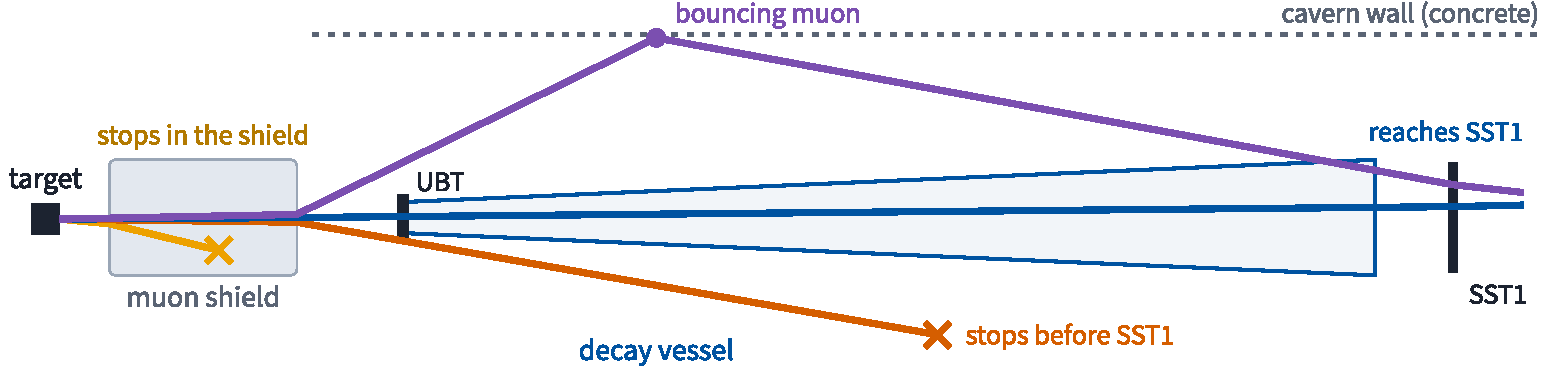
\includegraphics[width=1.00\linewidth,height=59.18pt,keepaspectratio]{figs/s38_sk1.pdf}\par}
\vspace{2.46pt}
\noindent \begin{minipage}[t]{\dimexpr(0.5000\linewidth-0.5000\dimexpr11.49pt\relax)}\vspace{0pt}\raggedright
{\fontsize{5.71pt}{7.42pt}\selectfont\setlength{\tabcolsep}{4.00pt}\renewcommand{\arraystretch}{1.42}
\begin{tabular}{lr}
\textcolor{muted}{Nov-4 muon category (type)} & \textcolor{muted}{per spill} \\\headrule
stop before z = 30.6 m (shield, TCC8 rock) & 4.38×10\textsuperscript{10} \\\rowrule
fly past the vessel / into the hall walls & 2.42×10\textsuperscript{9} \\\rowrule
stop between 30.6 and 82 m (cavern rock) & 6.75×10\textsuperscript{8} \\\rowrule
in the rock at 82 m & 1.48×10\textsuperscript{7} \\\rowrule
cross the vessel region, miss SST1 & 2.49×10\textsuperscript{4} \\\rowrule
\rowcolor{tint}\bfseries SST1, bounced off the cavern wall / floor & \bfseries 1.09×10\textsuperscript{4} \\\rowrule
\rowcolor{tint}\bfseries SST1, straight, good track (p > 1 GeV, 4 stations + TD) & \bfseries 6.05×10\textsuperscript{3} \\\rowrule
\rowcolor{tint}\bfseries SST1, other (soft or outside the stations / TD) & \bfseries 1.49×10\textsuperscript{4} \\\rowrule
\end{tabular}\par}
\end{minipage}%
\hfill%
\begin{minipage}[t]{\dimexpr(0.5000\linewidth-0.5000\dimexpr11.49pt\relax)}\vspace{0pt}\raggedright
{\fontsize{6.15pt}{8.60pt}\selectfont
\begin{itemize}
  \item Every muon is followed from the target to z = 30.6 m and to SST1; its type is set by where it ends
  \item \textbf{Bounced}: leave the vessel region, scatter in the cavern concrete and come back into SST1; their straight backward line misses the planes they crossed (bounce search)
  \item \textbf{Straight, p > 1 GeV, 4 straw stations + TD}: the good tracks of the pair candidates
\end{itemize}}
\end{minipage}\par
\end{btframe}

% ---------------------------------------------------------------- slide 39b: Nov-4 muon flux vs 2018 (19 Nov 2026)
\begin{btframe}{7 · Back-up · muon flux vs 2018}{Muon flux at the target: Nov-4 production vs the 2018 FairShip sample}
{\centering 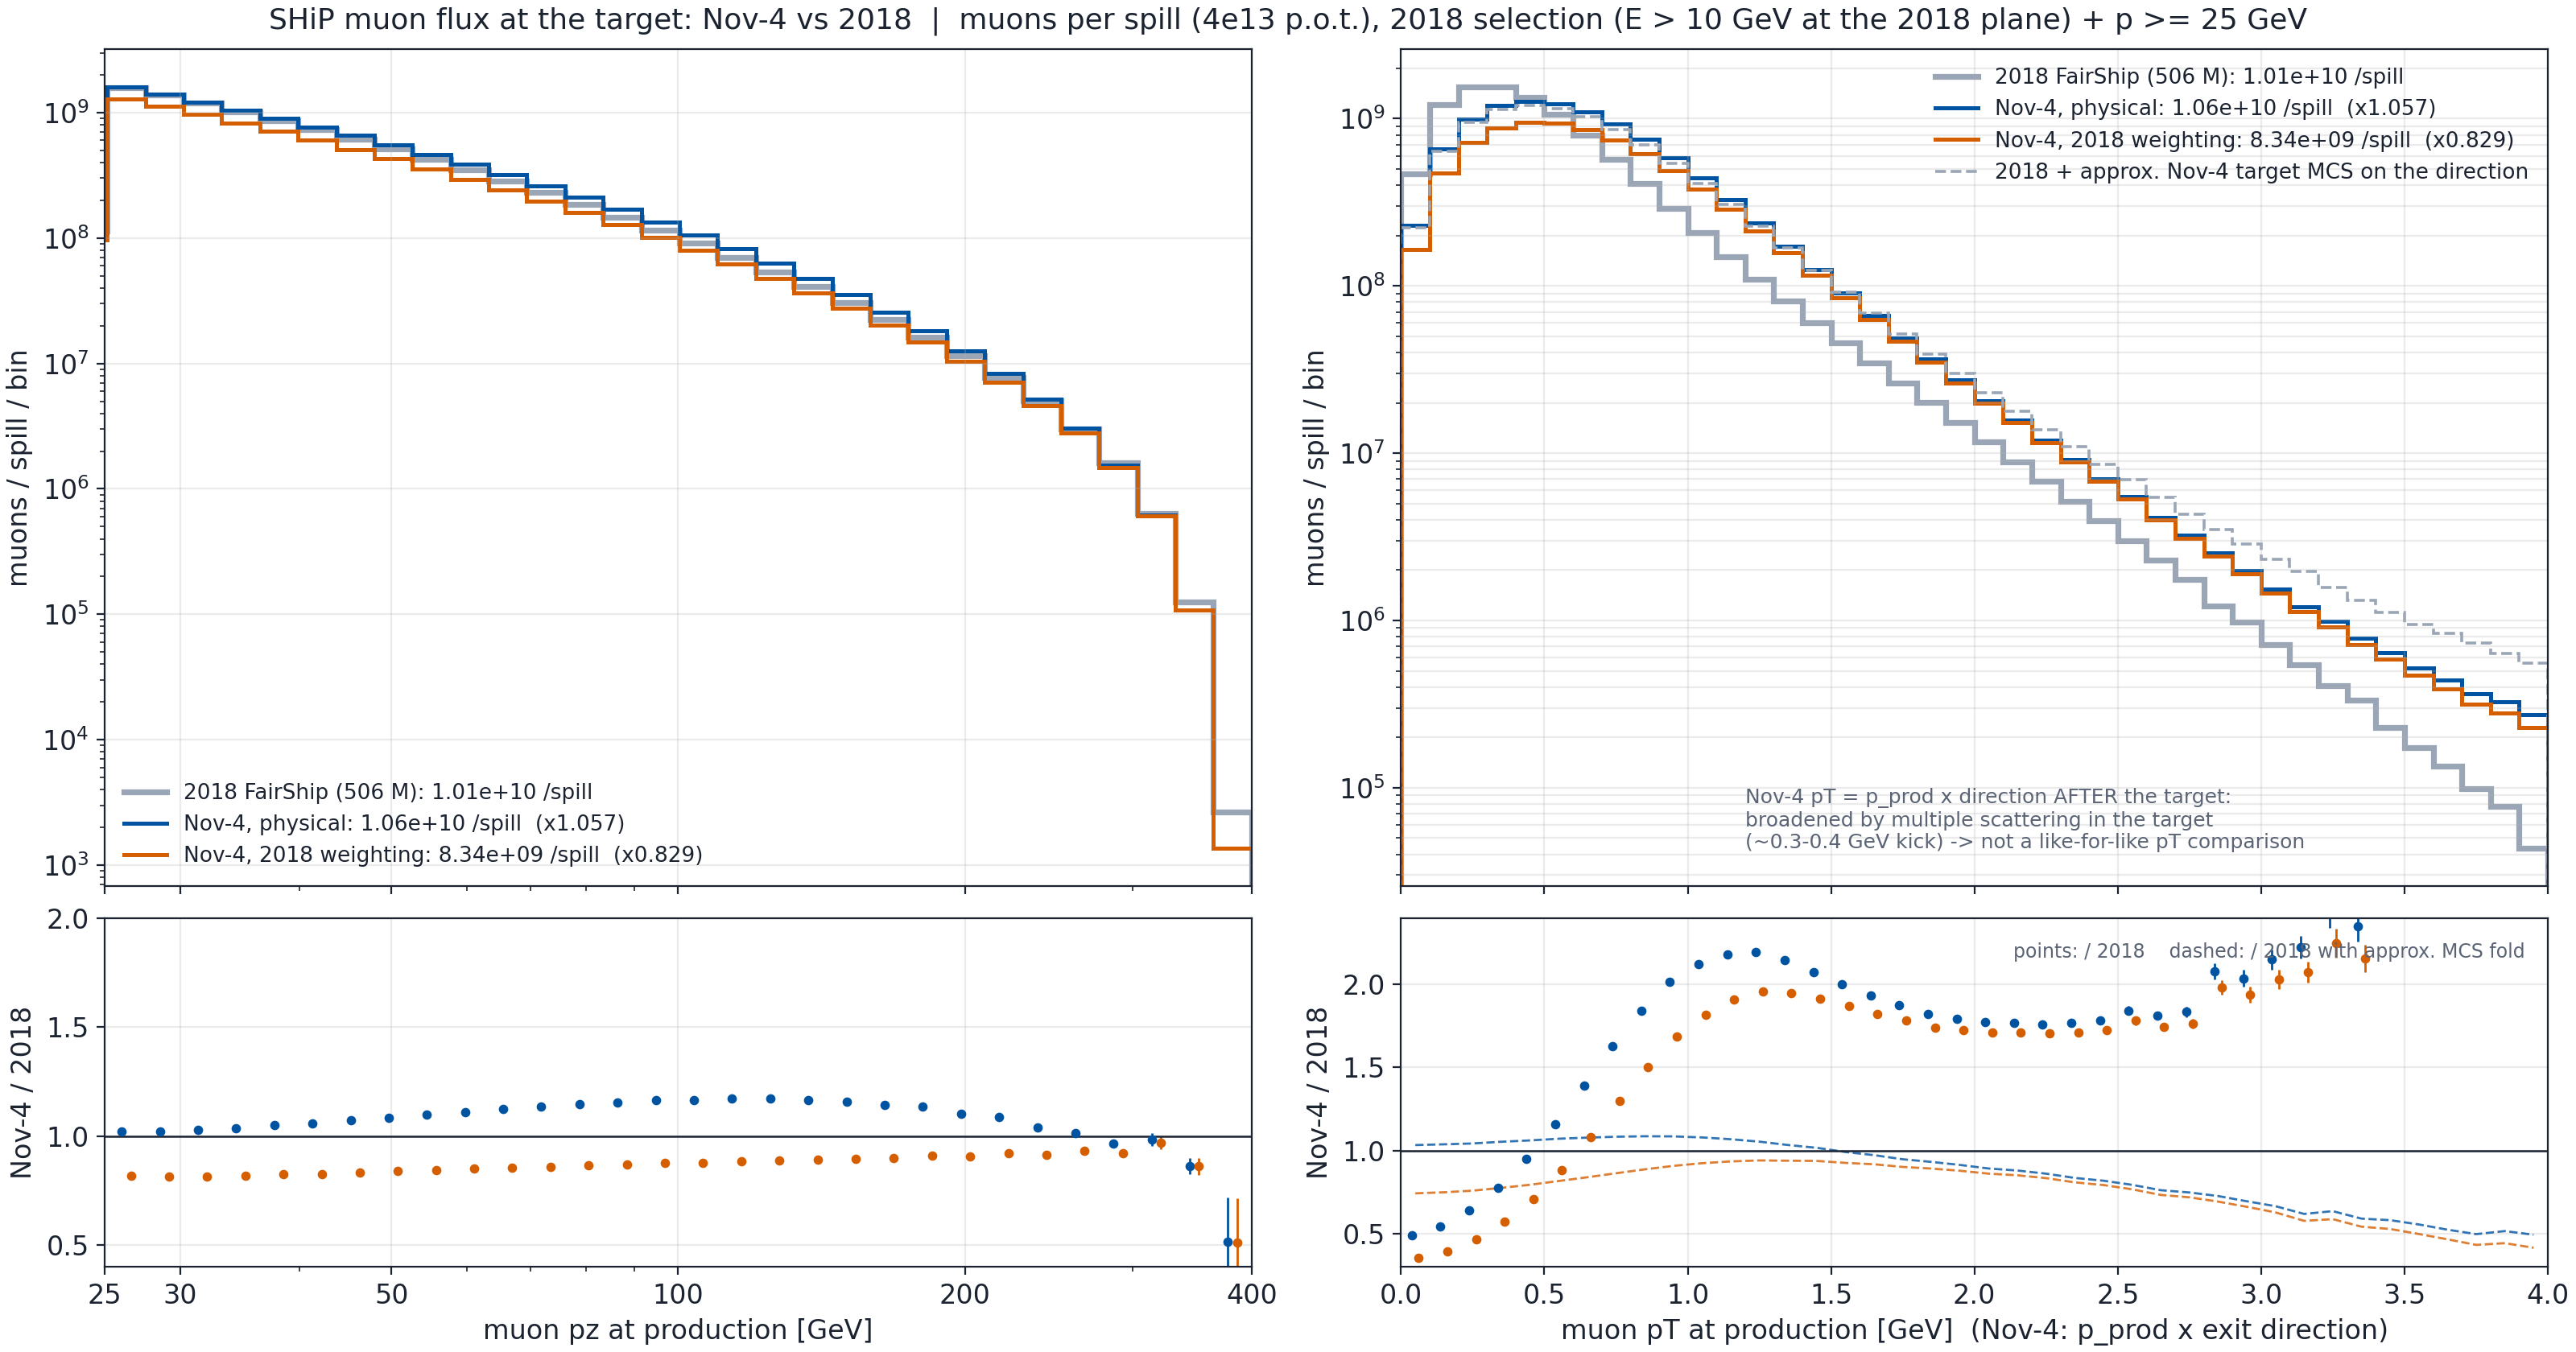
\includegraphics[height=138pt,keepaspectratio]{figs/s39b_nov4_vs_2018.png}\par}
\vspace{1.5pt}
{\fontsize{5.9pt}{8.0pt}\selectfont
\begin{itemize}
  \item Same 2018 selection on both (E > 10 GeV at the 2018 plane, p ≥ 25 GeV): Nov-4 / 2018 = \textbf{1.057}; charm, beauty, onia 0.98–1.00
  \item With FairShip's \textbf{2018 weighting emulated} (η → μμγ, ω → π\textsuperscript{0}μμ muons /100 without the ×100 boost): \textbf{0.83} → the 2018 files lack \textasciitilde{}22–27 \% of the min-bias flux
  \item p\textsubscript{T} is not like-for-like: Nov-4 keeps only the direction after the target (dashed: 2018 with approximate target scattering)
\end{itemize}}
\end{btframe}

% ---------------------------------------------------------------- 23 Nov 2026: how the cavern-rock x mu pairs form (4-station + TD good track, preliminary)
\begin{btframe}{7 · Back-up · cavern-rock × μ pairs}{Cavern-rock × μ pairs: where the vertex is and which particles (4 stations + TD, DOCA < 1 cm)}
\noindent \begin{minipage}[t]{\dimexpr(0.50\linewidth-0.50\dimexpr9.67pt\relax)}\vspace{0pt}\centering
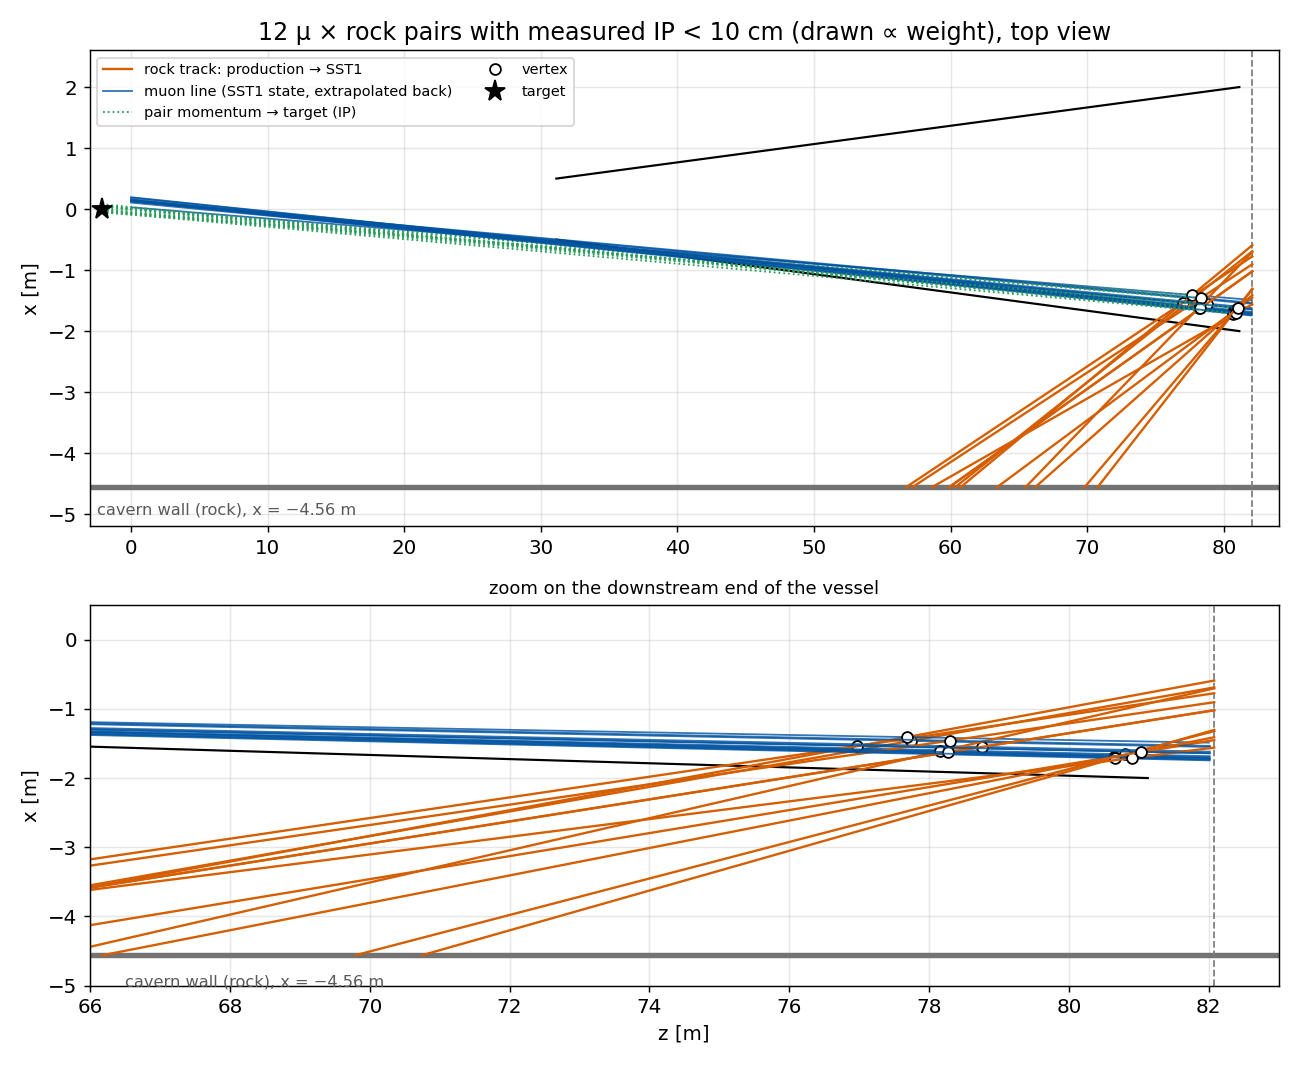
\includegraphics[width=\linewidth,height=165pt,keepaspectratio]{figs/s47_rock_mu_pairs_doca1.png}\par
\end{minipage}%
\hfill%
\begin{minipage}[t]{\dimexpr(0.50\linewidth-0.50\dimexpr9.67pt\relax)}\vspace{0pt}\raggedright
\begin{itemize}
  \item \textbf{Rock leg:} soft negative hadron (median 1.8 GeV) from the −x cavern wall at z ≈ 59–69 m, entering the vessel through the −x wall
  \item \textbf{Muon leg:} hard μ\textsuperscript{+} (median 222 GeV) along the −x wall; alone it misses the target by +18 cm
  \item \textbf{Vertex:} large opening angle (220 mrad) → closest approach just inside the −x wall, z ≈ 77–81 m; the rock leg tilts the pair onto the target (+3 cm)
\end{itemize}
\vspace{2pt}
{\fontsize{5.02pt}{6.52pt}\selectfont\setlength{\tabcolsep}{3.2pt}\renewcommand{\arraystretch}{1.42}
\begin{tabularx}{\linewidth}{>{\raggedright\arraybackslash}Xrrrr}
\textcolor{muted}{pairs / 15 y, before tagging (PDG μ, rock)} & \textcolor{muted}{w\textsubscript{μ} / spill} & \textcolor{muted}{w\textsubscript{rock} / spill} & \textcolor{muted}{IP < 10 cm} & \textcolor{muted}{share} \\\headrule
μ\textsuperscript{+} × π\textsuperscript{−} (−13, −211) & 0.0025 & 4.6 & 30.9 & 73 \% \\\rowrule
μ\textsuperscript{+} × K\textsuperscript{−} (−13, −321) & 0.0025 & 4.5 & 5.7 & 14 \% \\\rowrule
μ\textsuperscript{+} × p̄ (−13, −2212) & 0.0025 & 4.4 & 3.2 & 8 \% \\\rowrule
μ\textsuperscript{+} × e\textsuperscript{−} (−13, 11) & 0.0025 & 4.9 & 2.0 & 5 \% \\\rowrule
μ\textsuperscript{−} × positive (13, +) & & & 0.05 & 0 \\\rowrule
\rowcolor{tint}\bfseries total (candidates 110, IP < 2.5 m 108) & & & \bfseries 42 & \\\rowrule
\end{tabularx}\par}
\vspace{2pt}
\begin{itemize}
  \item 4 stations + TD on both legs, DOCA < 1 cm, all muons: 110 / 42 / 108 per 15 y (DOCA < 2 cm: 220 / 84 / 216; old SST1 + TD: 634 / 211 / 626); weights = median per leg
  \item After tagging: R1 0.097 ± 0.012, R2 < 0.027 (90 \% CL), Z1 1.2×10\textsuperscript{-5}
\end{itemize}
\end{minipage}\par
\end{btframe}

% ---------------------------------------------------------------- 24 Nov 2026: cavern-rock x mu vertices with the pair lines, and vertex z (4-station + TD, preliminary)
\begin{btframe}{7 · Back-up · cavern-rock × μ vertices}{Cavern-rock × μ vertices in the vessel (4 stations + TD, DOCA < 1 cm)}
\centering
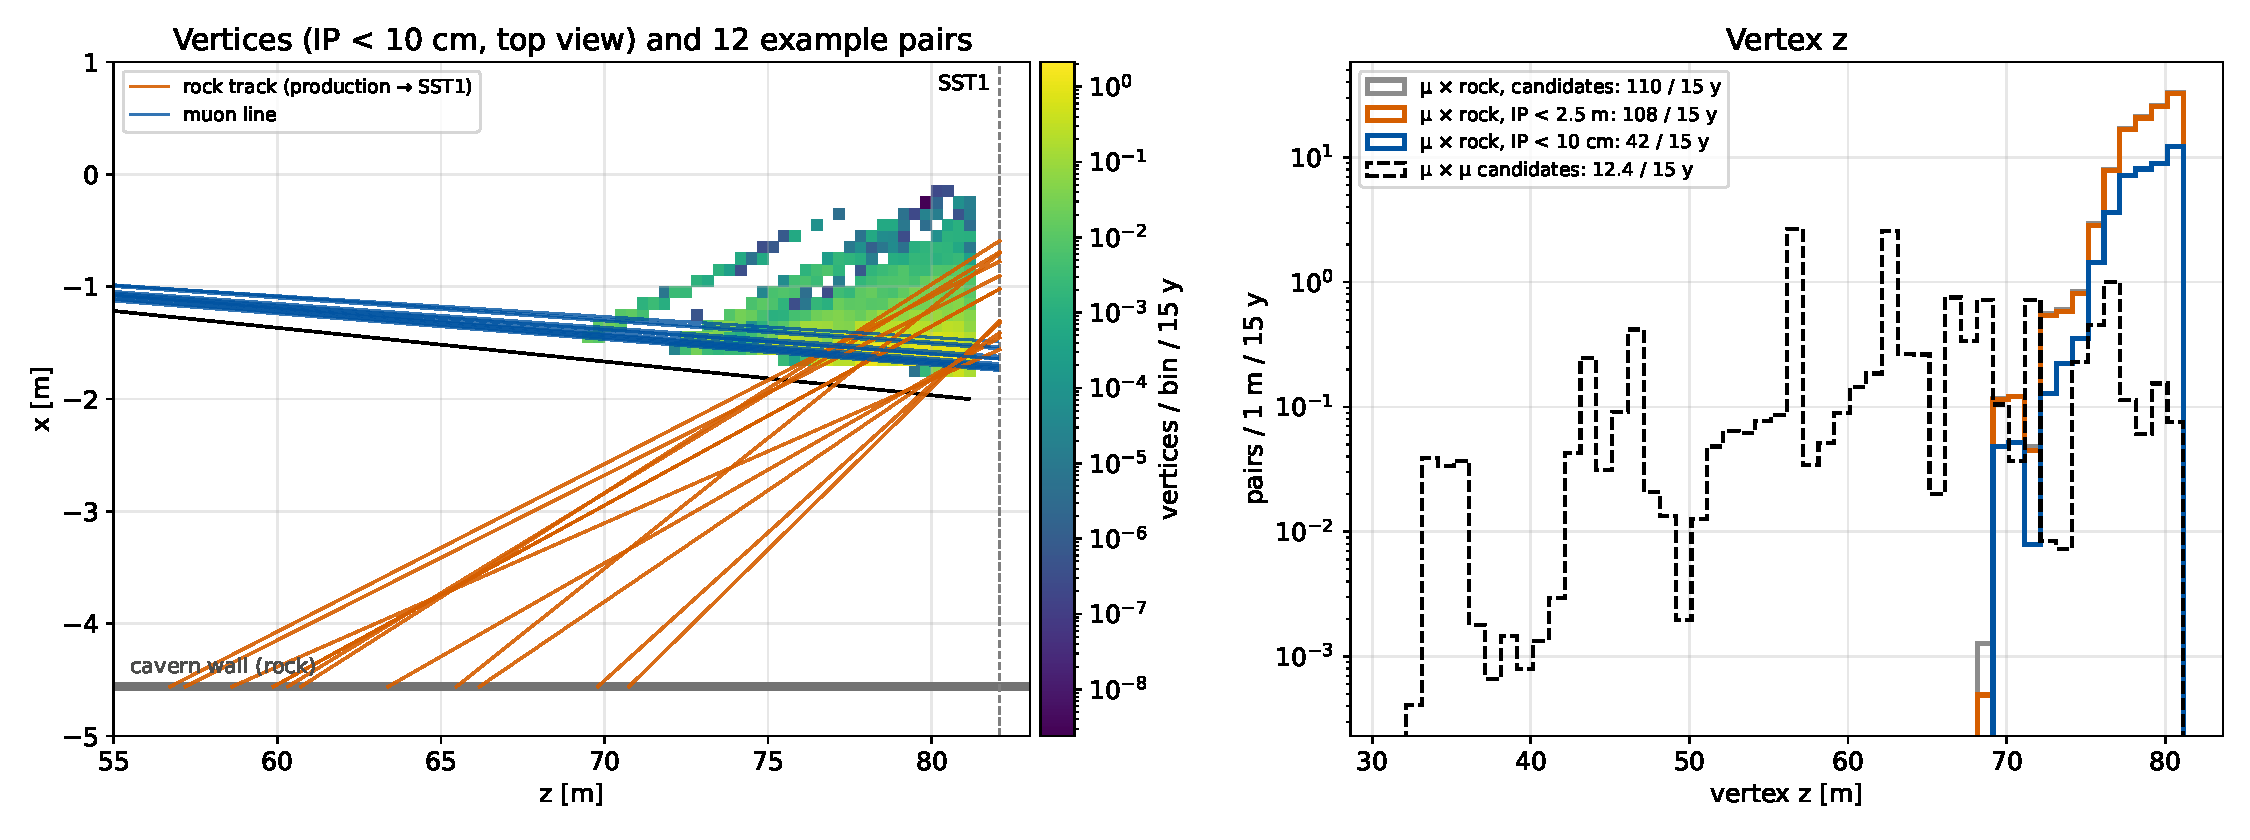
\includegraphics[width=0.96\linewidth,height=170pt,keepaspectratio]{figs/s48_rock_mu_vertices_doca1.pdf}\par
\vspace{4pt}
\raggedright
\begin{itemize}\footnotesize
  \item Left: vertices of the pairs with measured IP < 10 cm (top view, per 15 y) and 12 example pairs: rock tracks (orange) from the −x cavern wall cross the muon lines (blue) just inside the −x vessel wall
  \item Right: vertex z at each cut, μ × μ for comparison: all μ × rock vertices in the last ~10 m of the vessel (median 79.1 m), μ × μ spread over the whole vessel
\end{itemize}
\end{btframe}
% ---------------------------------------------------------------- back-up: x-z maps of the combinatorial pair vertices (24 Nov 2026)
\begin{btframe}{7 · Back-up · combinatorial vertices}{Where the combinatorial vertices are: MS7 interaction × μ and cavern rock × μ (DOCA < 1 cm)}
\centering
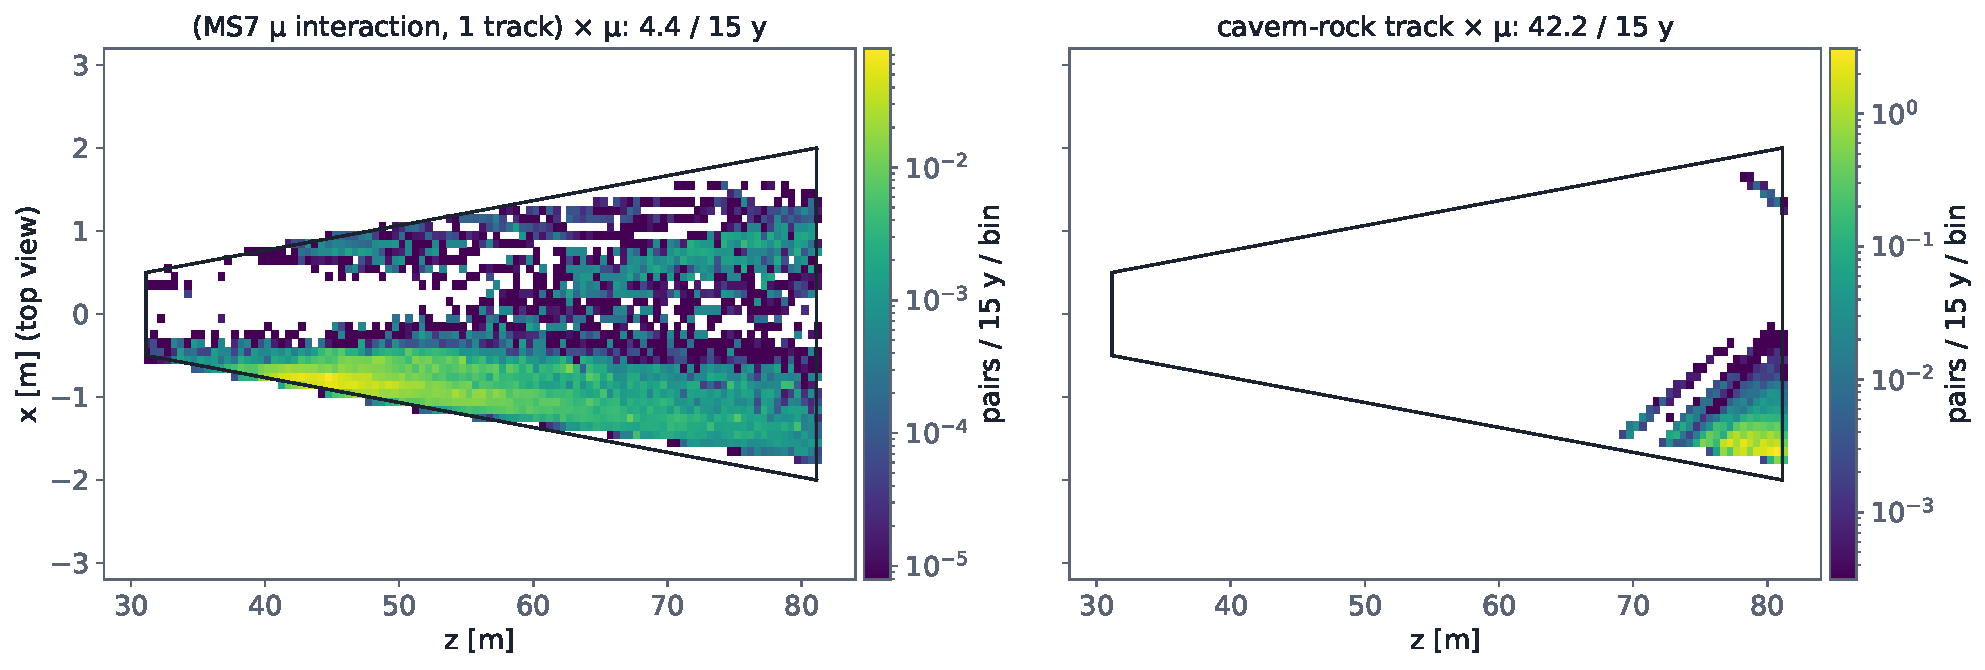
\includegraphics[width=\linewidth,height=150pt,keepaspectratio]{figs/s20_pairs_xz_doca1.pdf}\par
\vspace{4pt}
\raggedright
\begin{itemize}\footnotesize
  \item Top view of the pair vertices with measured IP < 10 cm, per 15 y, 4-station good track; vessel outline in black
  \item MS7 interaction (1 track) × μ: 4.4 / 15 y, spread over the whole vessel near the −x wall; cavern rock × μ: 42 / 15 y, last ~10 m, −x side
\end{itemize}
\end{btframe}

% ---------------------------------------------------------------- slide 40: MS7 KL: from production to SST1, and the comparison with data
\begin{btframe}{7 · Back-up · MS7 K\textsubscript{L}}{MS7 K\textsubscript{L}: from production to SST1, and the comparison with data}
\noindent \begin{minipage}[t]{\dimexpr(0.5556\linewidth-0.5556\dimexpr9.67pt\relax)}\vspace{0pt}\raggedright
{\fontsize{5.02pt}{6.52pt}\selectfont\setlength{\tabcolsep}{3.51pt}\renewcommand{\arraystretch}{1.42}
\begin{tabularx}{\linewidth}{>{\raggedright\arraybackslash}Xrr}
\textcolor{muted}{step} & \textcolor{muted}{per spill} & \textcolor{muted}{note} \\\headrule
muons crossing the last 50 cm of MS7 & 4.6×10\textsuperscript{8} & Nov-4 transport \\\rowrule
muon interactions (Geant4 muonNuclear) & 8.0×10\textsuperscript{5} & P ≈ 1.7×10\textsuperscript{-3} per muon \\\rowrule
K\textsubscript{L} made (vertex 7.8×10\textsuperscript{3} + shower 7.6×10\textsuperscript{3}) & 1.5×10\textsuperscript{4} & 0.0099 per interaction at the vertex \\\rowrule
K\textsubscript{L} leaving the iron (T > 0.5 GeV) & 3.2×10\textsuperscript{3} & absorption λ ≈ 19 cm \\\rowrule
K\textsubscript{L} decaying in the vessel & 1.5×10\textsuperscript{3} – 2.0×10\textsuperscript{3} & 49 \% of those leaving \\\rowrule
\rowcolor{tint}\bfseries two good tracks, pair cuts (DOCA < 1 cm) & \bfseries 0.78 & \bfseries 1.17×10\textsuperscript{7} / 15 y \\\rowrule
\rowcolor{tint}\bfseries IP < 10 cm (full selection) & \bfseries 8.1×10\textsuperscript{-4} & \bfseries 1.22×10\textsuperscript{4} / 15 y \\\rowrule
\end{tabularx}\par}
\end{minipage}%
\hfill%
\begin{minipage}[t]{\dimexpr(0.4444\linewidth-0.4444\dimexpr9.67pt\relax)}\vspace{0pt}\raggedright
{\fontsize{5.02pt}{6.52pt}\selectfont\setlength{\tabcolsep}{3.51pt}\renewcommand{\arraystretch}{1.42}
\begin{tabularx}{\linewidth}{>{\raggedright\arraybackslash}Xrrr}
\textcolor{muted}{V0 per event, W = 6.2 GeV} & \textcolor{muted}{K\textsubscript{S}} & \textcolor{muted}{Λ (+Σ\textsuperscript{0})} & \textcolor{muted}{Λ̄} \\\headrule
γp, E\textsubscript{γ} = 20 GeV (SLAC) & 0.082 ± 0.003 & 0.049 ± 0.002 & 0.0029 ± 0.0003 \\\rowrule
\rowcolor{tint}\bfseries Geant4 11.2 muonNuclear & \bfseries 0.087 & \bfseries 0.051 & \bfseries 0.0020 \\\rowrule
Pythia 6 & 0.153 & 0.090 & 0.0058 \\\rowrule
\end{tabularx}\par}
\vspace{2.46pt}
{\fontsize{4.78pt}{6.45pt}\selectfont Geant4 reproduces the measured K\textsubscript{S} and Λ yields within 6 \% at W = 6.2 GeV; Pythia 6 is ×1.9 high. Most MS7 K\textsubscript{L} come from W = 5–10 GeV; low W (1.6–3 GeV) is not yet compared (ISSUES D16).\par}
\end{minipage}\par
\end{btframe}

% ---------------------------------------------------------------- slide 40q: Q2 and W of the interactions that make the MS7 KL (19 Nov 2026)
\begin{btframe}{7 · Back-up · MS7 K\textsubscript{L} production}{Which muon interactions make the MS7 K\textsubscript{L}: Q\textsuperscript{2} and W}
\begin{minipage}[t]{0.27\linewidth}\vspace{0pt}\centering
{\fontsize{5.5pt}{6.5pt}\selectfont Geant4 11.2 muonNuclear (default)\par}
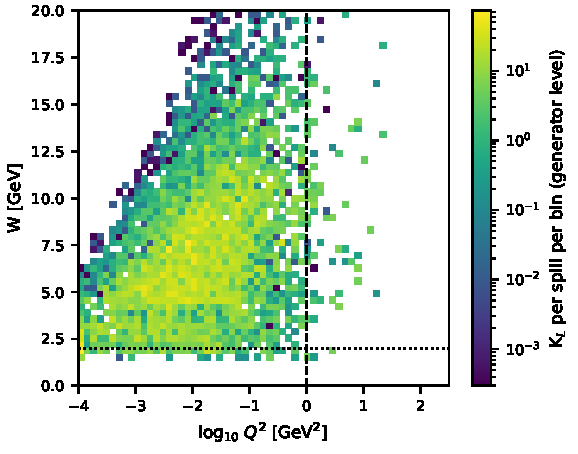
\includegraphics[width=\linewidth]{figs/kl_q2w_geant4.pdf}
\end{minipage}\hfill
\begin{minipage}[t]{0.27\linewidth}\vspace{0pt}\centering
{\fontsize{5.5pt}{6.5pt}\selectfont Pythia 6\par}
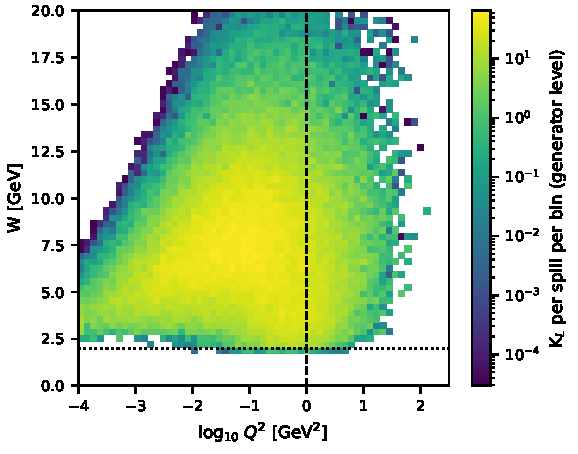
\includegraphics[width=\linewidth]{figs/kl_q2w_pythia6.pdf}
\end{minipage}\hfill
\begin{minipage}[t]{0.42\linewidth}\vspace{0pt}
{\fontsize{5.9pt}{7.9pt}\selectfont
\begin{itemize}
  \item Geant4: 96 \% of the interactions have Q\textsuperscript{2} < 0.1 GeV\textsuperscript{2} and 72 \% W < 2 GeV, but they make almost no K\textsubscript{L}
  \item \textcolor{cern}{\textbf{The K\textsubscript{L} come from W = 5–10 GeV (55 \%) and W > 10 GeV (15 \%)}}: 5 \% of the interactions, still at Q\textsuperscript{2} < 1 GeV\textsuperscript{2} (98 \%)
  \item Pythia 6 fills the same region but makes ≈ 14× more K\textsubscript{L} per interaction there
  \item \textbf{Quasi-real photoproduction at W ≈ 3–10 GeV}, where γp data exist: used to choose the generator (next slides)
\end{itemize}}
\end{minipage}
\vspace{2pt}
{\centering 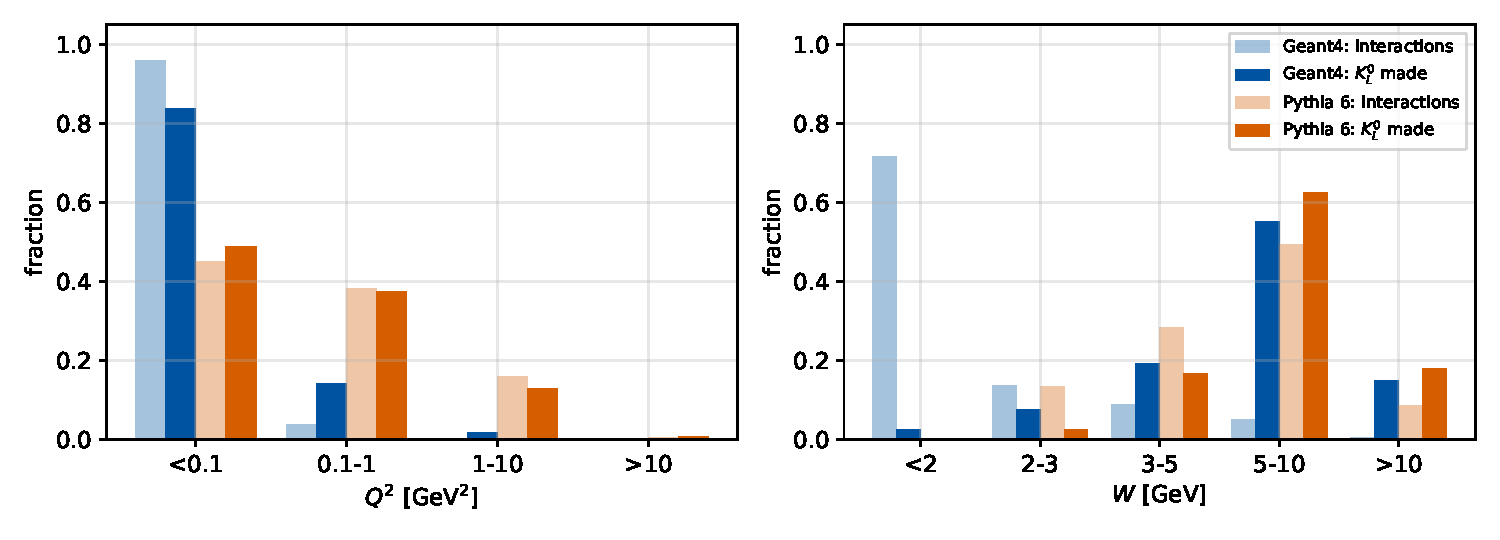
\includegraphics[width=0.80\linewidth,height=88pt,keepaspectratio]{figs/int_kl_q2w_shares.pdf}\par}
\begin{tikzpicture}[remember picture,overlay]
\node[anchor=north east,inner sep=0] (t1) at ([xshift=-14pt,yshift=-6pt]current page.north east) {
\includegraphics[width=125pt]{figs/talk_2.png}};
\end{tikzpicture}
\end{btframe}

% ---------------------------------------------------------------- slide 40a1: MS7 KL production, Geant4 vs Pythia vs data (19 Nov 2026)
\begin{btframe}{7 · Back-up · MS7 K\textsubscript{L} production}{MS7 K\textsubscript{L}: what we know, Geant4 and Pythia against the data}
{\centering 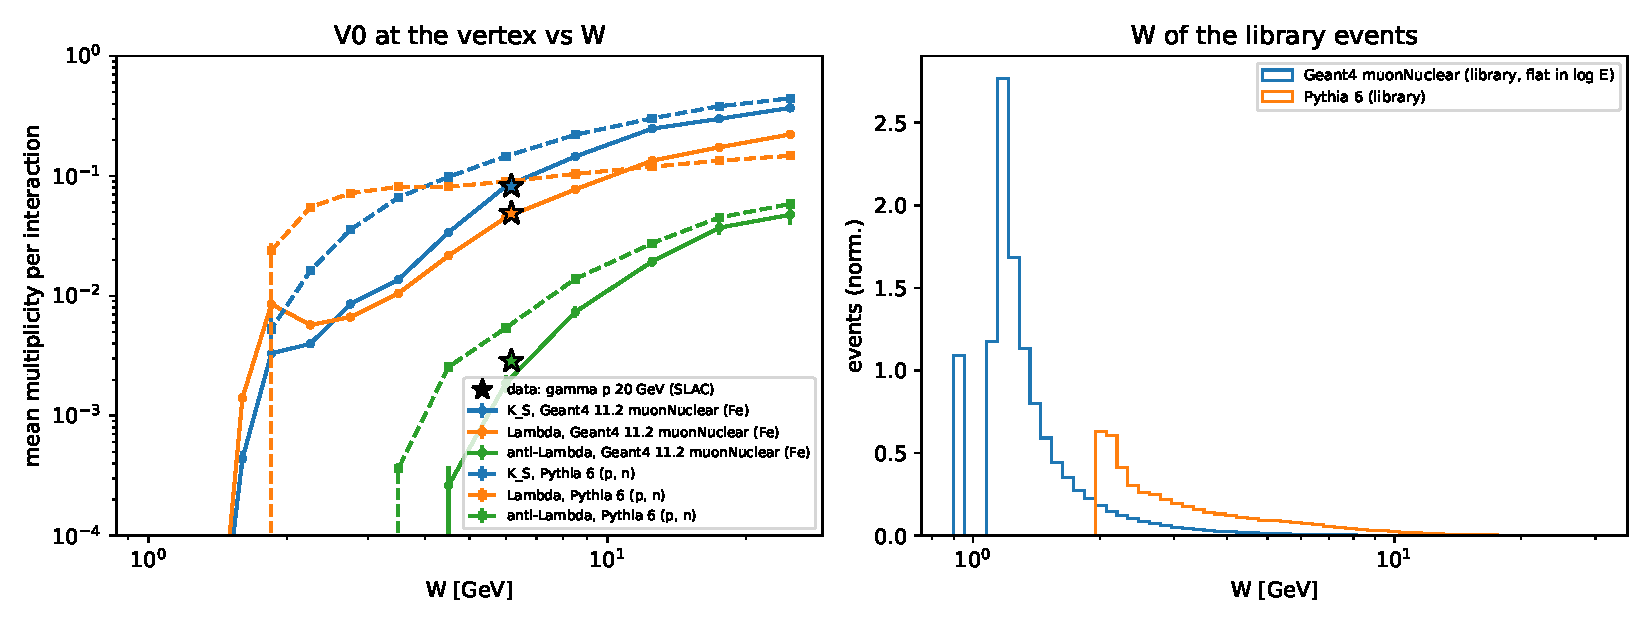
\includegraphics[width=0.86\linewidth,height=118pt,keepaspectratio]{figs/v0_vs_W.pdf}\par}
\vspace{2.46pt}
{\fontsize{5.9pt}{7.9pt}\selectfont
\begin{itemize}
  \item \textbf{Generators:} \textcolor{cern}{\textbf{Geant4 11.2 muonNuclear}} on Fe (default; median W 1.3 GeV, mostly below the K Λ threshold) and \textbf{Pythia 6.4.28} γ\textsuperscript{*} on p, n (W > 2 GeV only). Per interaction: K\textsubscript{L} 0.0099 (Geant4) vs 0.12 (Pythia), mostly from their different W spectra (right)
  \item \textbf{K\textsubscript{L} is not measured directly:} K\textsuperscript{0}, \=K\textsuperscript{0} give ½ K\textsubscript{S} + ½ K\textsubscript{L}, so K\textsubscript{L} = K\textsubscript{S} and the K\textsubscript{S} data validate it
  \item \textbf{Data:} SLAC γp at E\textsubscript{γ} = 20 GeV (W = 6.2 GeV, stars): K\textsubscript{S} 0.082 ± 0.003, Λ 0.049 ± 0.002 per event. \textcolor{cern}{\textbf{Geant4 within 6 \%}}, Pythia ×1.9 high. Cross-check: NOMAD ν\textsubscript{μ} CC on C, K\textsubscript{S} 0.068 per event
  \item \textbf{Chain (per spill):} 1.5×10\textsuperscript{4} K\textsubscript{L} made (half by the shower in the iron) → 3.2×10\textsuperscript{3} leave the iron (37 \% from the shower) → 1.5×10\textsuperscript{3} decay in the vessel. Geant4 11.4 and 11.2 agree within 1–3 \%
\end{itemize}}
\slidenote{Data: K. Abe et al., PRD 30 (1984) 1 (SLAC SHF, Table II); NOMAD: P. Astier et al., NPB 621 (2002) 3.}
\end{btframe}

% ---------------------------------------------------------------- slide 40a2: MS7 KL production at low W (19 Nov 2026)
\begin{btframe}{7 · Back-up · MS7 K\textsubscript{L} production}{Strangeness at low W: where most Geant4 interactions are}
{\centering 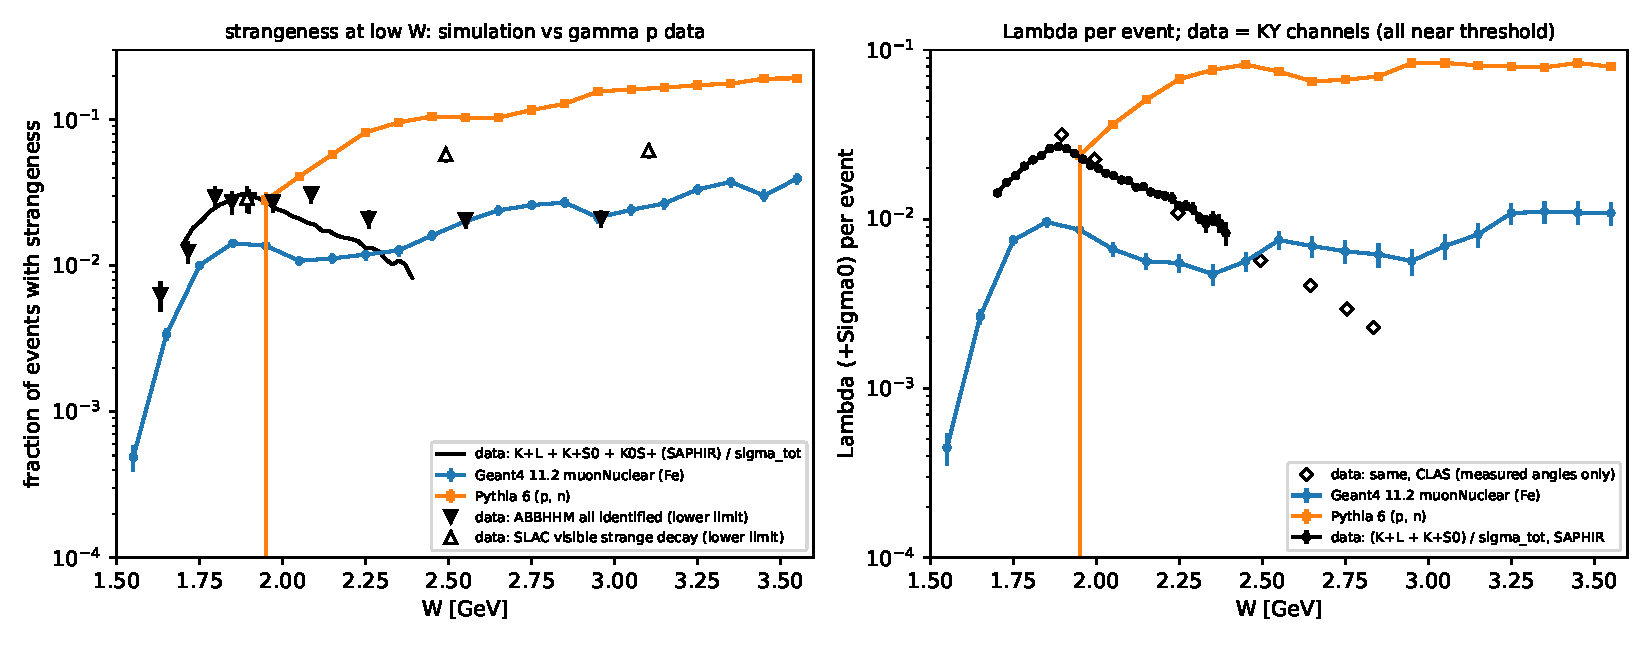
\includegraphics[width=0.86\linewidth,height=118pt,keepaspectratio]{figs/v0_lowW.pdf}\par}
\vspace{2.46pt}
{\fontsize{5.9pt}{7.9pt}\selectfont
\begin{itemize}
  \item \textbf{Data (γp, near threshold, all lower limits):} SAPHIR and CLAS exclusive K Λ, K Σ cross sections over σ\textsubscript{tot}; ABBHHM identified strange final states; SLAC visible strange decays
  \item Geant4 is \textbf{low by ≥ ×2} for W < 2.2 GeV and by ≥ ×2.5–3 at W = 2.5–3 GeV; Pythia (W > 2 GeV) is ×3–5 above the exclusive Λ channels
  \item \textbf{Impact is small:} of the vertex K\textsubscript{L} that can leave the iron (T > 0.5 GeV), \textcolor{cern}{\textbf{78 \% come from W > 5 GeV}} (validated, previous slide), 14 \% from 3.5–5 GeV, 7.6 \% from W < 3.5 GeV. A ×2–3 deficit there gives \textbf{+8–15 \%} on the K\textsubscript{L}
  \item \textbf{Open:} W = 3.5–5 GeV not compared with data (14 \% of the relevant K\textsubscript{L}); the selected K\textsubscript{L} rest on 74 simulated events
\end{itemize}}
\slidenote{Data: SAPHIR (Glander 2004, Lawall 2005), CLAS (McCracken 2010, Dey 2010; measured angles only), ABBHHM (Erbe 1969), SLAC (Ballam 1969, Bingham 1973); σ\textsubscript{tot}: Armstrong 1972, Caldwell 1973.}
\end{btframe}

% ---------------------------------------------------------------- slide 40b: MS7 KL momentum, decay point and SST1 (19 Nov 2026)
\begin{btframe}{7 · Back-up · MS7 K\textsubscript{L} momentum}{MS7 K\textsubscript{L}: momentum at the decay point and of its charged products at SST1}
\begin{minipage}[t]{0.49\linewidth}\vspace{0pt}\centering
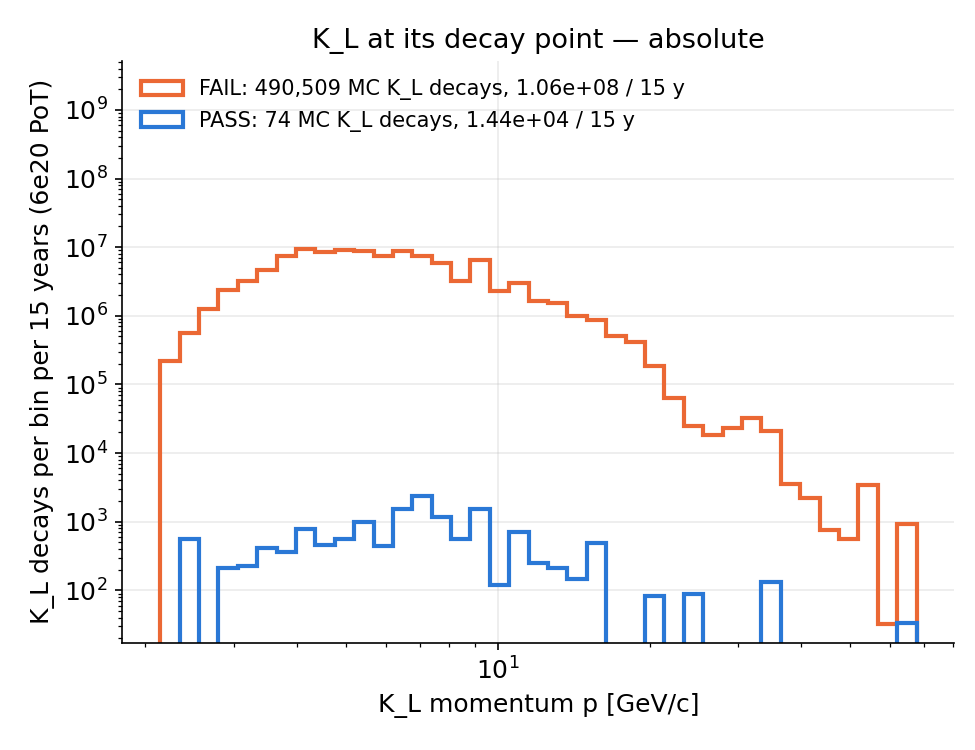
\includegraphics[width=0.84\linewidth]{figs/s40b_kl_p.png}
\end{minipage}\hfill
\begin{minipage}[t]{0.49\linewidth}\vspace{0pt}\centering
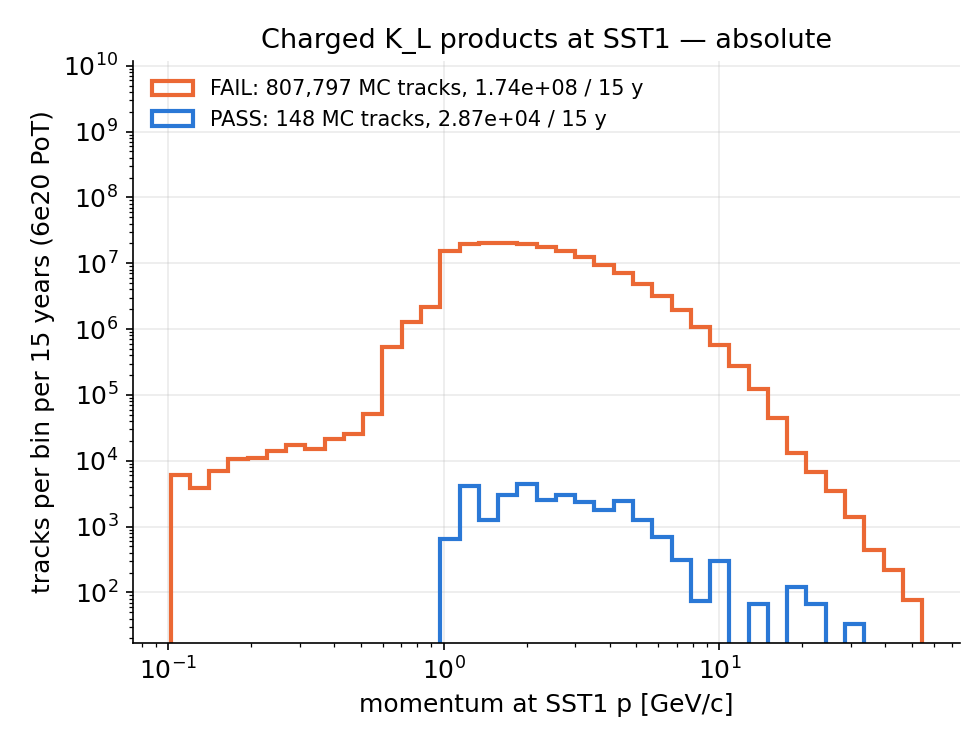
\includegraphics[width=0.84\linewidth]{figs/s40b_sst1_p.png}
\end{minipage}
\vspace{2.46pt}
{\fontsize{6.15pt}{8.60pt}\selectfont
\begin{itemize}
  \item \textcolor{cern}{\textbf{PASS}} the full selection: 74 simulated decays, 1.44×10\textsuperscript{4} / 15 y; \textbf{FAIL}: 4.9×10\textsuperscript{5} decays, 1.06×10\textsuperscript{8} / 15 y
  \item Selected K\textsubscript{L} are slightly harder (median 6.8 vs 5.6 GeV: \textbf{β = 0.9974} vs 0.9960, 0.36 ns behind light over 40 m) and decay further downstream (median z 72 vs 65 m)
  \item At SST1 the selected events have exactly two charged tracks, median 2.3 GeV (2.0 GeV for FAIL); none below the 1 GeV cut
\end{itemize}}
\end{btframe}

% ---------------------------------------------------------------- slide 40c: MS7 KL species, decay point and SST1 (19 Nov 2026)
\begin{btframe}{7 · Back-up · MS7 K\textsubscript{L} species}{MS7 K\textsubscript{L}: particles at the decay point and at SST1}
\begin{minipage}[t]{0.49\linewidth}\vspace{0pt}\centering
{\fontsize{5.5pt}{7pt}\selectfont\textcolor{muted}{at the decay point}\par}
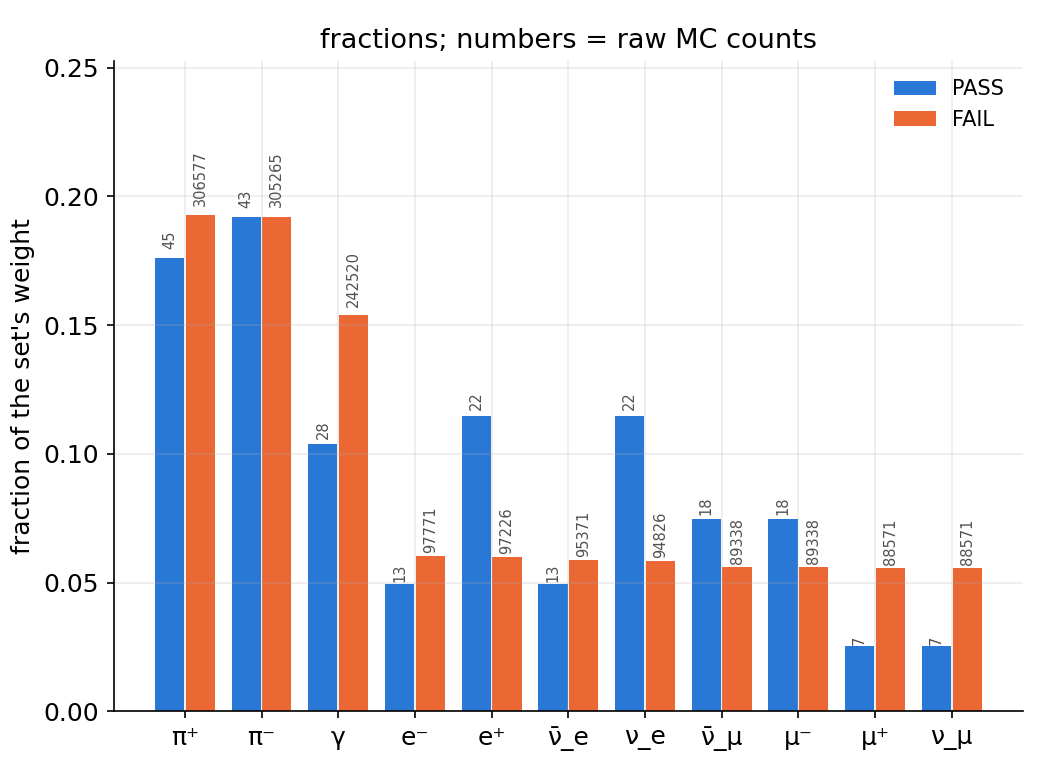
\includegraphics[width=0.92\linewidth]{figs/s40c_pdg_decay.png}
\end{minipage}\hfill
\begin{minipage}[t]{0.49\linewidth}\vspace{0pt}\centering
{\fontsize{5.5pt}{7pt}\selectfont\textcolor{muted}{K\textsubscript{L} products reaching SST1}\par}
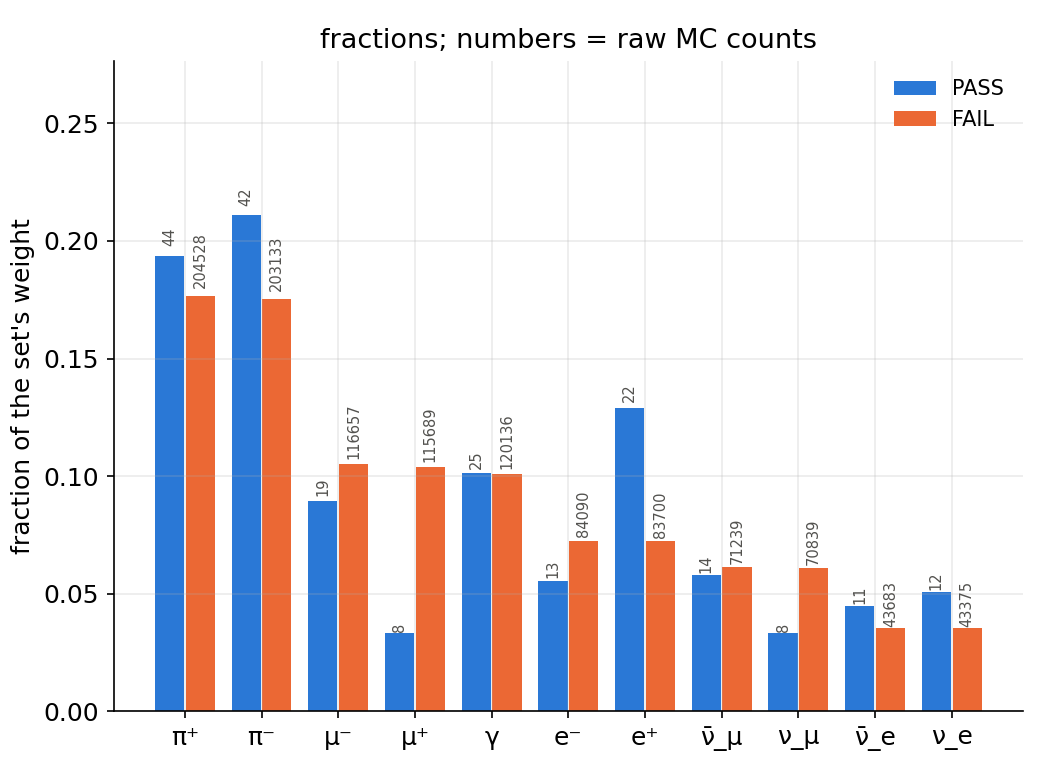
\includegraphics[width=0.92\linewidth]{figs/s40c_pdg_sst1.png}
\end{minipage}
\vspace{2.46pt}
{\fontsize{6.15pt}{8.60pt}\selectfont
\begin{itemize}
  \item Selected decays are mostly semileptonic: K\textsubscript{e3} 52 \%, K\textsubscript{μ3} 32 \%, π\textsuperscript{+}π\textsuperscript{−}π\textsuperscript{0} 16 \% (FAIL follows the decay table: π\textsuperscript{+}π\textsuperscript{−}π\textsuperscript{0} 25 \%)
  \item At SST1 the pions dominate both sets (\textasciitilde{}20 \% each charge); the e\textsuperscript{+} excess and μ\textsuperscript{+} deficit of PASS are within its statistics (74 events)
\end{itemize}}
\end{btframe}


% ---------------------------------------------------------------- slide 40d: Q2 and W of the parent interaction, PASS vs FAIL (20 Nov 2026)
\begin{btframe}{7 · Back-up · MS7 K\textsubscript{L} parent DIS}{MS7 K\textsubscript{L}: Q\textsuperscript{2} and W of the muon interaction that made it, PASS vs FAIL}
{\centering 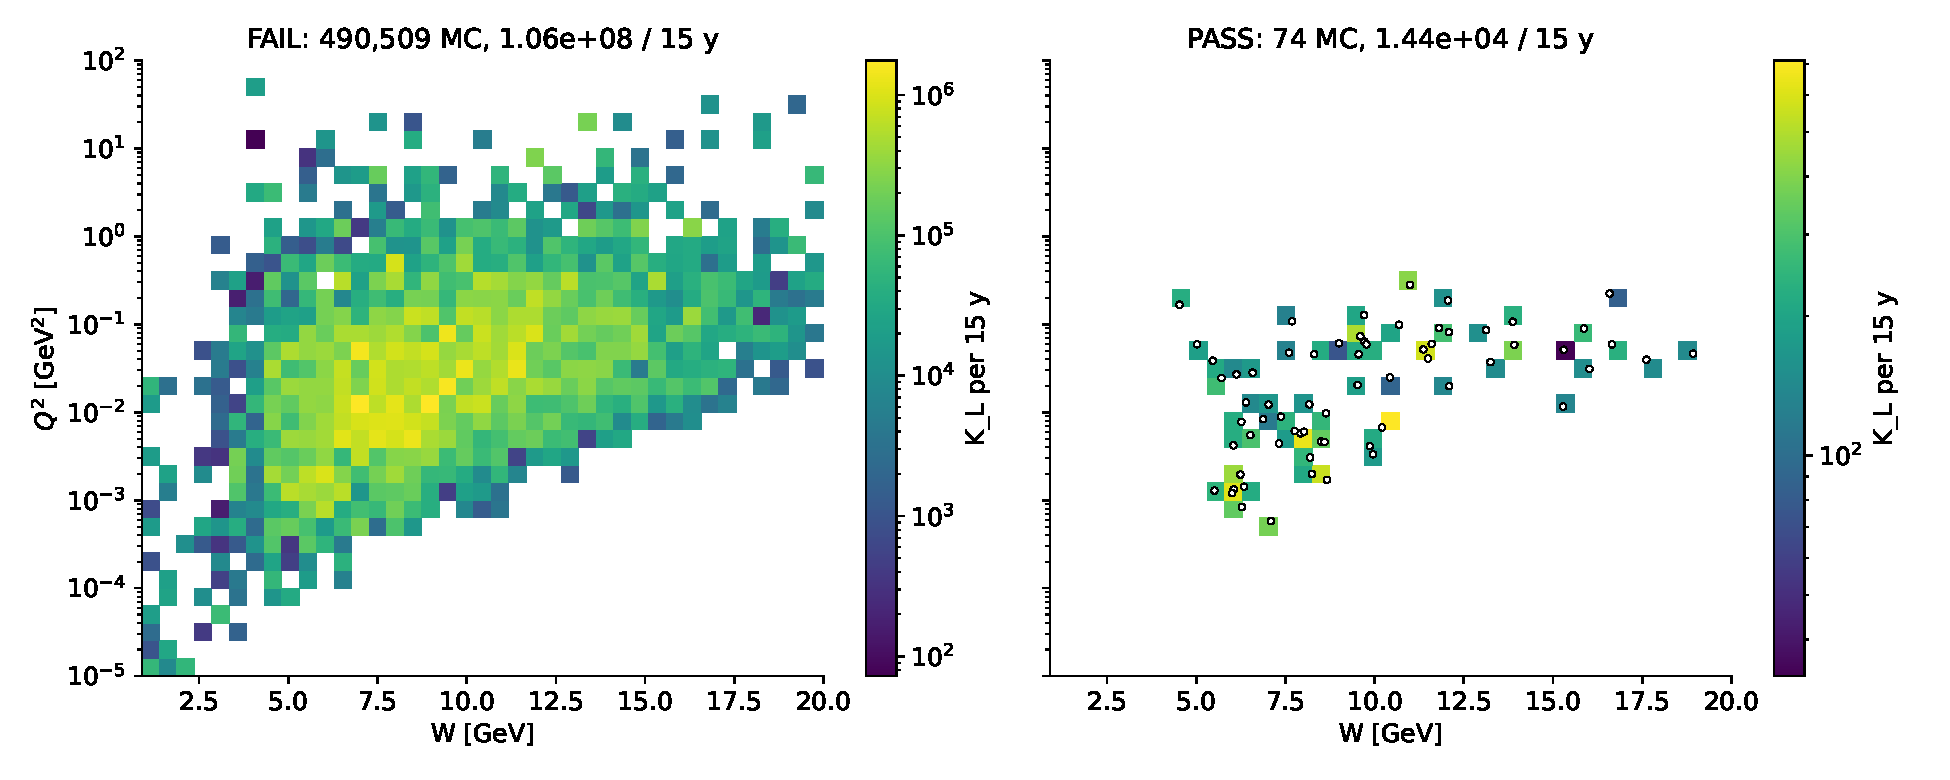
\includegraphics[width=0.80\linewidth,height=100pt,keepaspectratio]{figs/s40d_kl_q2_vs_w.pdf}\par}
\vspace{2pt}
\begin{minipage}[t]{0.52\linewidth}\vspace{0pt}
{\fontsize{5.02pt}{6.52pt}\selectfont\setlength{\tabcolsep}{3.51pt}\renewcommand{\arraystretch}{1.30}
\begin{tabularx}{\linewidth}{>{\raggedright\arraybackslash}Xrrr}
\textcolor{muted}{weighted, per 15 y} & \textcolor{muted}{PASS} & \textcolor{muted}{FAIL} & \textcolor{muted}{all MS7 μ int.} \\\headrule
simulated / per 15 y & 74 / 1.44×10\textsuperscript{4} & 4.9×10\textsuperscript{5} / 1.06×10\textsuperscript{8} & 6×10\textsuperscript{7} / 1.4×10\textsuperscript{13} \\\rowrule
Q\textsuperscript{2} median [GeV\textsuperscript{2}] & 0.012 & 0.028 & 0.0011 \\\rowrule
Q\textsuperscript{2} < 0.01 / < 0.1 / > 1 GeV\textsuperscript{2} & 48 / 90 / 0 \% & 28 / 76 / 3.6 \% & 76 / 96 / 0.3 \% \\\rowrule
W median (10–90 \%) [GeV] & 8.6 (6.0–13.9) & 8.7 (5.7–13.4) & 1.5 (1.2–3.7) \\\rowrule
W < 3.5 / 3.5–5 / > 5 GeV & 0 / 1.6 / 98 \% & 0.6 / 4.3 / 95 \% & 89 / 5.4 / 5.6 \% \\\rowrule
ν / y / E\textsubscript{μ} median & 39 GeV / 0.29 / 122 GeV & 40 GeV / 0.40 / 106 GeV & 0.7 GeV / 0.017 / 70 GeV \\\rowrule
\end{tabularx}\par}
\end{minipage}\hfill
\begin{minipage}[t]{0.45\linewidth}\vspace{0pt}
{\fontsize{5.9pt}{7.9pt}\selectfont
\begin{itemize}
  \item \textcolor{cern}{\textbf{PASS and FAIL come from the same region: W > 5 GeV, quasi-real photon (Q\textsuperscript{2} < 0.1 GeV\textsuperscript{2})}}, ν ≈ 40 GeV: 5 \% of the MS7 interactions
  \item PASS is at \textbf{lower Q\textsuperscript{2} and y} and harder muons: a forward K\textsubscript{L} whose decay pair points back to the target (IP < 10 cm)
  \item No PASS event below W = 3.5 GeV: the data-poor low-W region does not affect the selected background
\end{itemize}}
\end{minipage}
\end{btframe}

% ---------------------------------------------------------------- slide 40e: who sees the parent (19 Nov 2026)
\begin{btframe}{7 · Back-up · MS7 K\textsubscript{L} parent}{Selected MS7 K\textsubscript{L}: which detector sees the parent interaction (R2, own hits only)}
{\centering 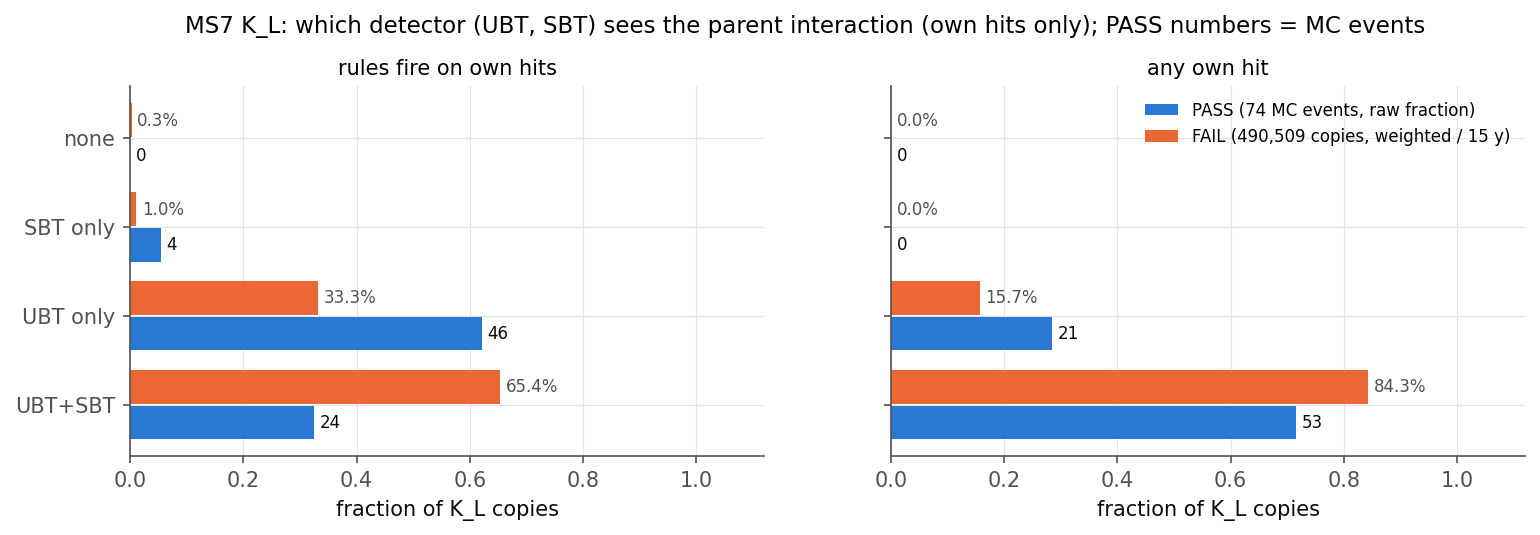
\includegraphics[width=0.84\linewidth]{figs/s40e_categories_nomsms.png}\par}
\vspace{2.46pt}
{\fontsize{6.15pt}{8.60pt}\selectfont
\begin{itemize}
  \item \textbf{UBT V0 rule tags 70 / 74} selected K\textsubscript{L} (FAIL 98.7 \%); the 4 it misses have p\textsubscript{vis} > 20 GeV (p\textsubscript{max} gate) and are tagged by the SBT
  \item SBT rules 28 / 74 (V0 line 18, zone 11, pointing 14); 4 are seen by the SBT only, 46 by the UBT only
  \item Every selected K\textsubscript{L} is tagged by the OR of the R2 rules (74 / 74; FAIL 99.7 \%)
\end{itemize}}
\end{btframe}

% ---------------------------------------------------------------- slide 40f: z dependence in MS7 (19 Nov 2026)
\begin{btframe}{7 · Back-up · MS7 K\textsubscript{L} production z}{Does it depend on where in MS7 the K\textsubscript{L} is made?}
{\centering 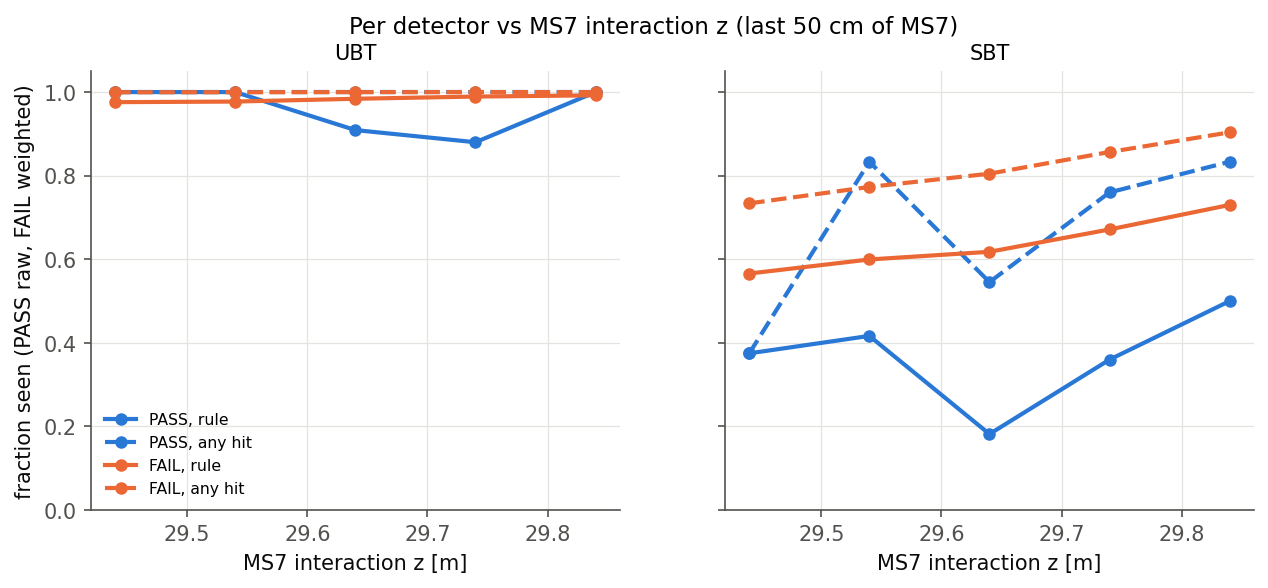
\includegraphics[width=0.90\linewidth,height=125pt,keepaspectratio]{figs/s40f_z_dependence_nomsms.png}\par}
\vspace{2.46pt}
{\fontsize{6.15pt}{8.60pt}\selectfont
\begin{itemize}
  \item \textbf{UBT}: any own hit 100 \% at every z; rule 88–100 \% (the misses are the p\textsubscript{vis} > 20 GeV events)
  \item \textbf{SBT}: more often seen for K\textsubscript{L} made at the end of the iron (FAIL 57 → 73 \%), probably because less iron is left to absorb the products (not yet checked)
  \item 95 \% of the K\textsubscript{L} come from the muon vertex itself (the rest from the shower, within 7 mm of it)
\end{itemize}}
\end{btframe}

% ---------------------------------------------------------------- slide 40d: V0-rule aperture (19 Nov 2026)
\begin{btframe}{7 · Back-up · V0 rule aperture}{V0-rule disc from the kinematic limit: r = 5 cm + p*\textsubscript{max} / p\textsubscript{vis} · Δz, p*\textsubscript{max} = 0.229 GeV}
\begin{minipage}[t]{0.49\linewidth}\vspace{0pt}\centering
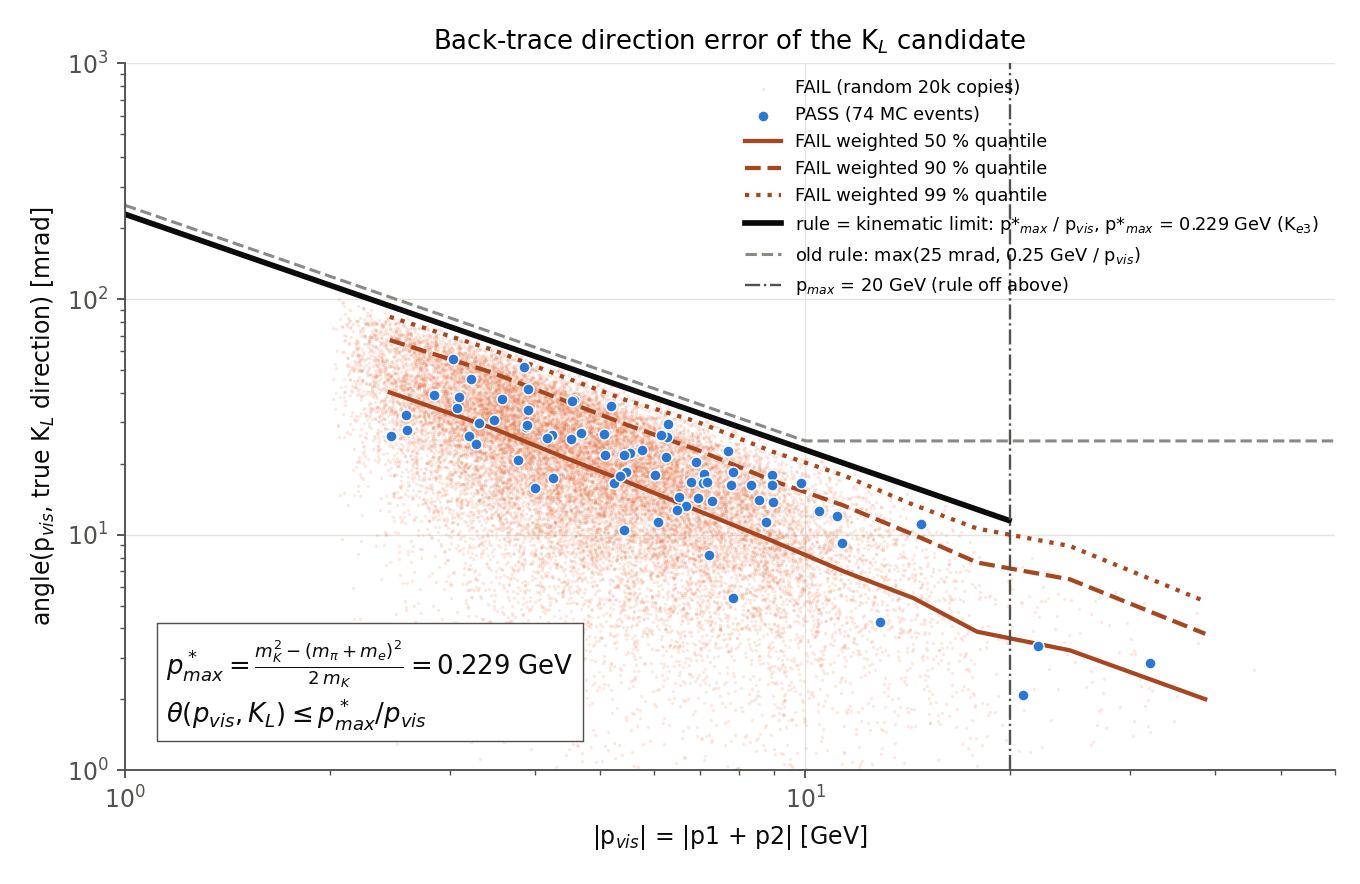
\includegraphics[width=0.88\linewidth]{figs/s40d_angle_vs_pvis_kin.png}
\end{minipage}\hfill
\begin{minipage}[t]{0.49\linewidth}\vspace{0pt}\centering
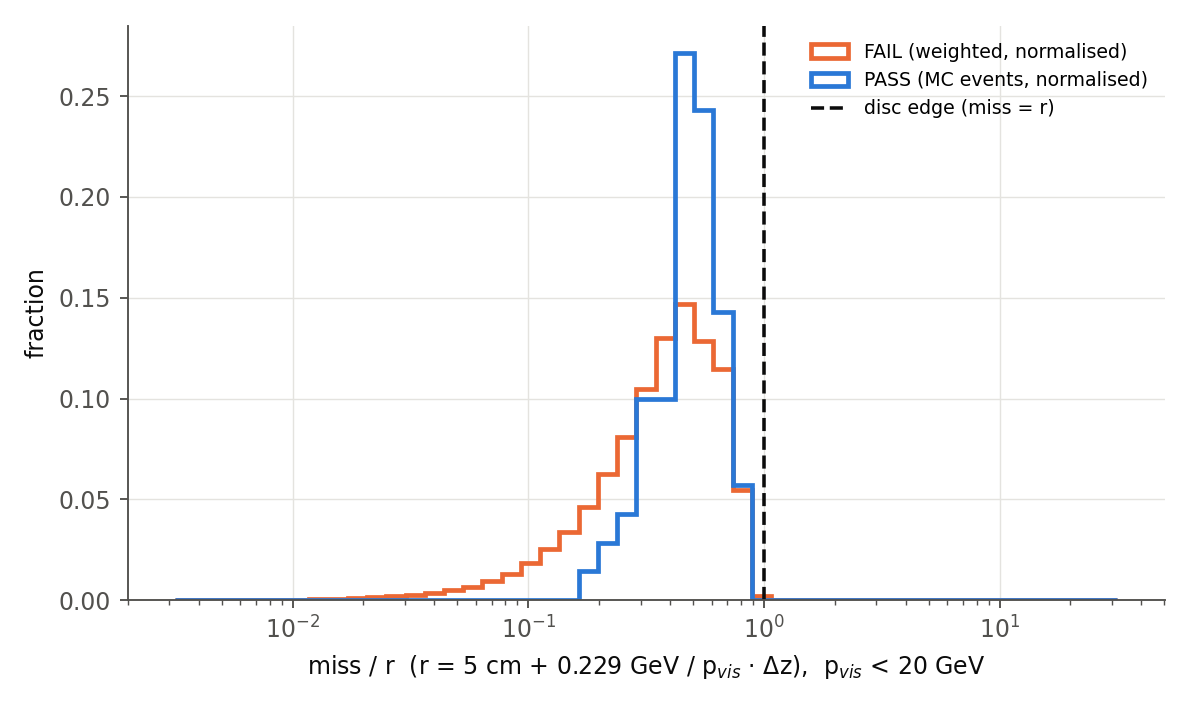
\includegraphics[width=0.88\linewidth]{figs/s40d_miss_over_r_kin.png}
\end{minipage}
\vspace{2.46pt}
{\fontsize{6.15pt}{8.60pt}\selectfont
\begin{itemize}
  \item The pair momentum p\textsubscript{vis} misses the K\textsubscript{L} direction because of the lost ν / π\textsuperscript{0}: selected median 18.5 mrad, 90 \% at 37 mrad; the error falls as 1/p
  \item Kinematic limit: in K\textsubscript{L} → π e ν the lost ν has at most \(p^*_{\max} = (m_K^2 - (m_\pi + m_e)^2)/2m_K\) = \textbf{0.229 GeV} (K\textsubscript{μ3} 0.188, π\textsuperscript{0} lost 0.132), so θ(p\textsubscript{vis}, K\textsubscript{L}) ≤ p*\textsubscript{max} / p\textsubscript{vis}; no tuned parameter, 5 cm = track-search radius
  \item All 4.9×10\textsuperscript{5} K\textsubscript{L} copies inside (max θ · p\textsubscript{vis} = 0.225 GeV). R2 test vs the old max(25 mrad, 0.25/p): MS7 0.81 → 0.84 / 15 y, signal lost 5.21 → 4.97 \% (20 k decays)
\end{itemize}}
\end{btframe}

% ---------------------------------------------------------------- slide 40r: search radius at the tile plane, track rule vs V0 rule (19 Nov 2026)
\begin{btframe}{7 · Back-up · search windows}{Search radius at the UBT tile plane: track rule and V0 rule}
{\centering 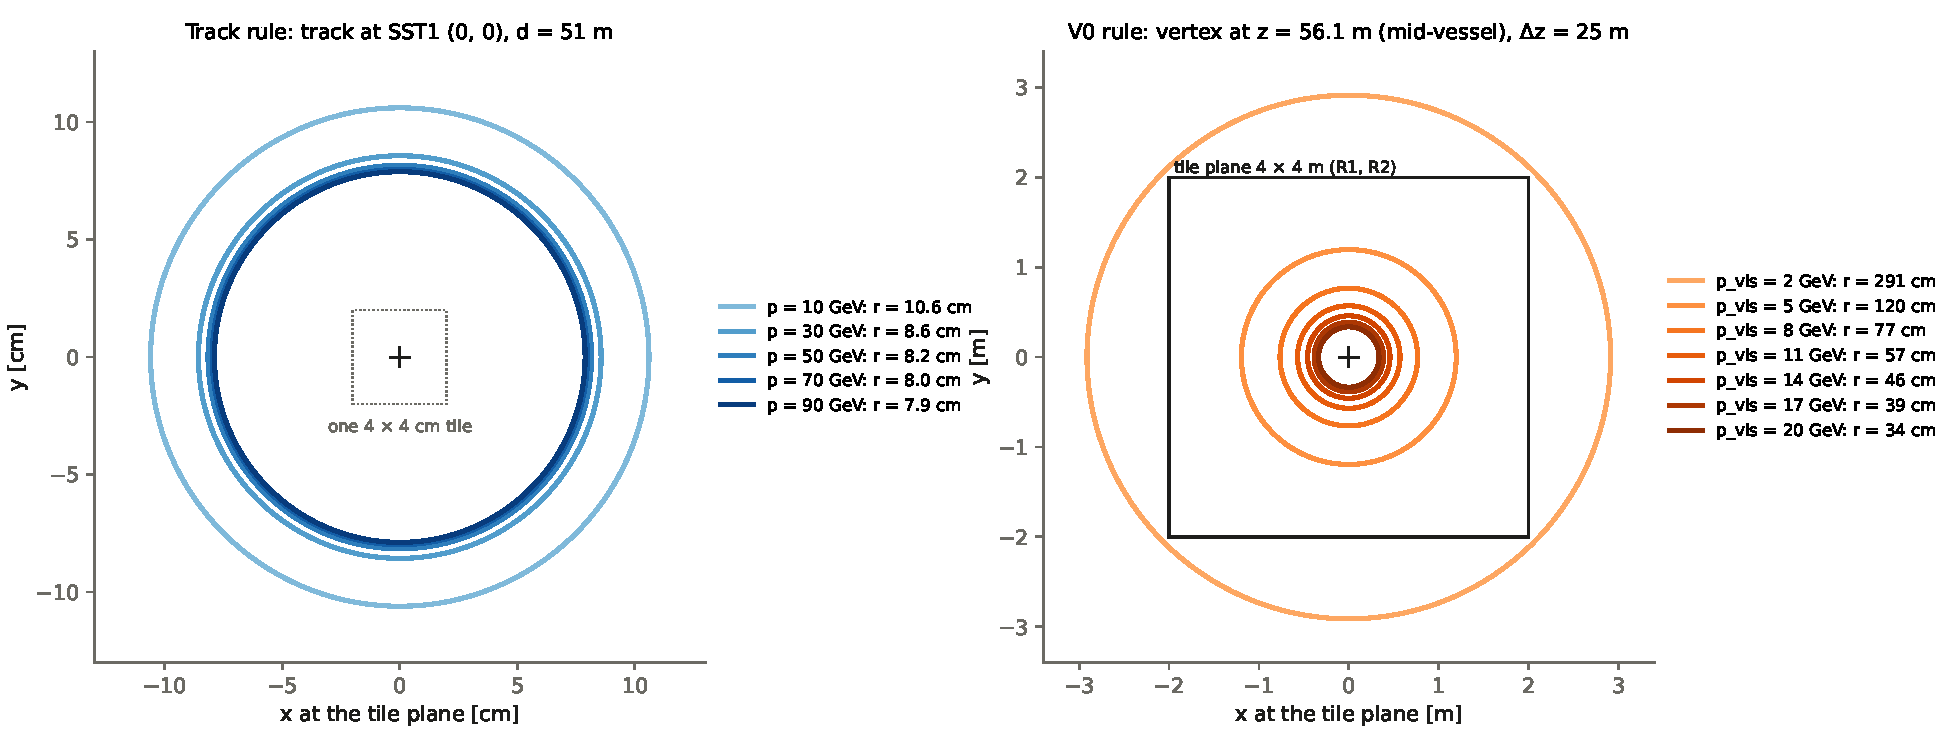
\includegraphics[width=\linewidth,height=136pt,keepaspectratio]{figs/aperture_radii_kin.pdf}\par}
\vspace{2.46pt}
{\fontsize{5.9pt}{7.9pt}\selectfont
\begin{itemize}
  \item \textbf{Track rule} (left), traced back from SST1 (82.08 m) over d = 51 m: r = 5 cm + (0.5 + 6 GeV / p) mrad × d → \textbf{10.6 cm at 10 GeV}, 7.9 cm at 90 GeV (straws, 30.73 m: +0.2 mm)
  \item \textbf{V0 rule} (right), vertex on axis in the middle of the vessel (z = 56.13 m, Δz = 25 m): r = 5 cm + 0.229 GeV / p\textsubscript{vis} × Δz → \textbf{2.9 m at 2 GeV}, 1.2 m at 5 GeV, 77 cm at 8 GeV, 46 cm at 14 GeV, \textbf{34 cm at 20 GeV}; the rule is off above p\textsubscript{vis} = 20 GeV
  \item The V0 disc is 3–30 × wider than a track window: it collects the most random hits, hence most of the signal loss (2 GeV: the disc covers the whole 4 × 4 m plane)
\end{itemize}}
\end{btframe}

% ---------------------------------------------------------------- slide 25: Slow MS7 KL escaped the 25 mrad cone: three fixes, A + C adopted
\begin{btframe}{7 · Back-up · V0 rule history}{Slow MS7 K\textsubscript{L} escaped the 25 mrad cone: three fixes, A + C adopted}
\noindent \begin{minipage}[t]{\dimexpr(0.2500\linewidth-0.2500\dimexpr14.22pt\relax)}\vspace{0pt}\raggedright
{\centering \fontsize{4.55pt}{6.15pt}\selectfont \textcolor{purple}{\textbf{25 mrad cone: misses (slow K\textsubscript{L})}}\par}
\vspace{0.27pt}
{\centering 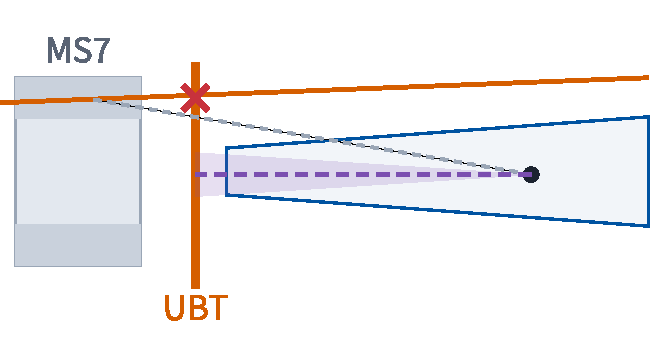
\includegraphics[width=1.00\linewidth,height=63.73pt,keepaspectratio]{figs/s24_sk1.pdf}\par}
\end{minipage}%
\hfill%
\begin{minipage}[t]{\dimexpr(0.2500\linewidth-0.2500\dimexpr14.22pt\relax)}\vspace{0pt}\raggedright
{\centering \fontsize{4.55pt}{6.15pt}\selectfont \textcolor{purple}{\textbf{A: cone max(25 mrad, 0.25 GeV / p\textsubscript{vis})}}\par}
\vspace{0.27pt}
{\centering 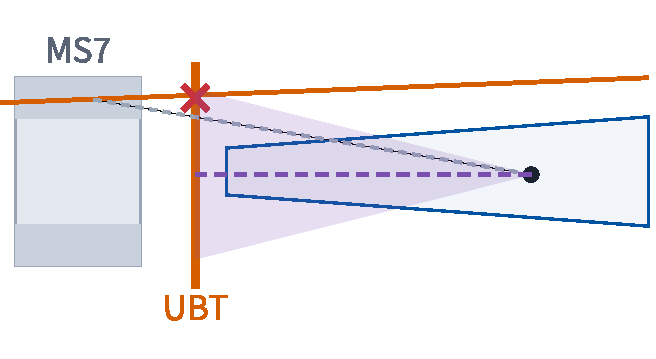
\includegraphics[width=1.00\linewidth,height=63.73pt,keepaspectratio]{figs/s24_sk2.pdf}\par}
\end{minipage}%
\hfill%
\begin{minipage}[t]{\dimexpr(0.2500\linewidth-0.2500\dimexpr14.22pt\relax)}\vspace{0pt}\raggedright
{\centering \fontsize{4.55pt}{6.15pt}\selectfont \textcolor{purple}{\textbf{B: extra lines to the yoke legs}}\par}
\vspace{0.27pt}
{\centering 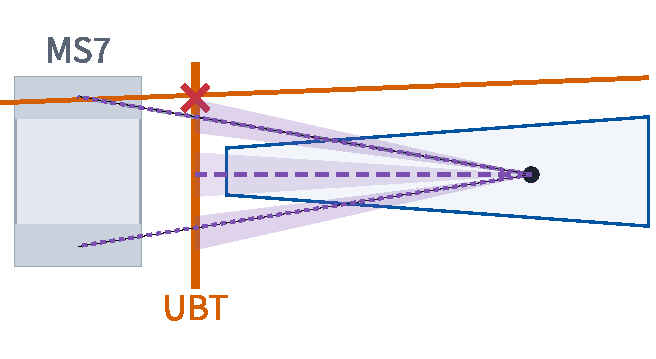
\includegraphics[width=1.00\linewidth,height=63.73pt,keepaspectratio]{figs/s24_sk3.pdf}\par}
\end{minipage}%
\hfill%
\begin{minipage}[t]{\dimexpr(0.2500\linewidth-0.2500\dimexpr14.22pt\relax)}\vspace{0pt}\raggedright
{\centering \fontsize{4.55pt}{6.15pt}\selectfont \textcolor{purple}{\textbf{C: window opened by the K\textsubscript{L} flight time}}\par}
\vspace{0.27pt}
{\centering 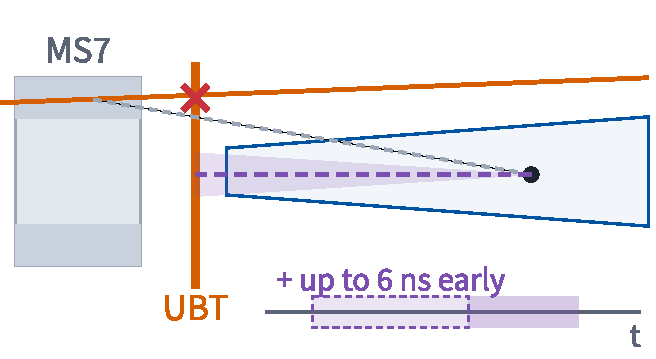
\includegraphics[width=1.00\linewidth,height=63.73pt,keepaspectratio]{figs/s24_sk4.pdf}\par}
\end{minipage}\par
\vspace{2.46pt}
{\fontsize{4.37pt}{5.68pt}\selectfont\setlength{\tabcolsep}{3.06pt}\renewcommand{\arraystretch}{1.42}
\begin{tabularx}{\linewidth}{>{\raggedright\arraybackslash}Xrrrr}
\textcolor{muted}{variant} & \textcolor{muted}{signal lost F / P} & \textcolor{muted}{MS7 μ tagged} & \textcolor{muted}{own hits only} & \textcolor{muted}{MS7 μ left / 15 y} \\\headrule
25 mrad (before the fix) & 5.3 / 9.4 \% & 66 \% & 63 \% & 8.1×10\textsuperscript{3} \\\rowrule
A: 1/p cone & 5.4 / 10.5 \% & 100 \% & 100 \% & 0.63 \\\rowrule
B: yoke lines & 12.1 / 25.1 \% & 100 \% & 100 \% & 0.48 \\\rowrule
C: time of flight & 4.9 / 7.6 \% & 68 \% & 67 \% & 7.8×10\textsuperscript{3} \\\rowrule
\rowcolor{tint}\bfseries A + C (adopted) & \bfseries 5.0 / 8.4 \% & \bfseries 100 \% & \bfseries 100 \% & \bfseries 0.67 \\\rowrule
B + C & 11.5 / 21.8 \% & 100 \% & 100 \% & 0.48 \\\rowrule
\end{tabularx}\par}
\end{btframe}

% 

% ---------------------------------------------------------------- slide 42: the OR of the rules (19 Nov 2026)
\begin{btframe}{7 · Back-up · OR of the rules}{All rules run on every candidate, in parallel: tagged = OR}
{\centering
\begin{tikzpicture}[x=1pt,y=1pt,font=\fontsize{5.2pt}{6.4pt}\selectfont,
  box/.style={line width=0.5pt,rounded corners=1.5pt,fill=white,align=center,inner sep=2.2pt,text width=140pt},
  arr/.style={-{Stealth[length=2.6pt]},line width=0.5pt,color=ink}]
  \node[draw=cern,fill=tint,line width=0.5pt,rounded corners=1.5pt,align=center,inner sep=2.5pt,text width=62pt] (c) at (0,0)
    {\textbf{\textcolor{cern}{candidate}}\\2 tracks at SST1\\vertex in the vessel};
  \node[box,draw=cern] (t) at (135,32) {\textbf{\textcolor{cern}{Track rule}} -- each track separately\\line from SST1 back\\r = 5 cm + (0.5 + 6 GeV/p) mrad · d};
  \node[box,draw=purple] (v) at (135,0) {\textbf{\textcolor{purple}{V0 rule}} -- the pair as one neutral (p\textsubscript{vis} < 20 GeV)\\line from the vertex along p\textsubscript{vis}, early time window};
  \node[box,draw=green] (s) at (135,-32) {\textbf{\textcolor{green}{SBT rules}} -- pointing, V0 line, zone};
  \node[circle,draw=ink,line width=0.6pt,fill=white,inner sep=1.2pt,font=\fontsize{6pt}{7pt}\selectfont\bfseries] (or) at (250,0) {OR};
  \node[draw=red,fill=red!8,line width=0.5pt,rounded corners=1.5pt,align=center,inner sep=2.5pt,text width=52pt] (out) at (310,0)
    {\textbf{\textcolor{red}{tagged}}\\any rule found a hit};
  \foreach \b in {t,v,s}{\draw[arr] (c.east) -- (\b.west); \draw[arr] (\b.east) -- (or);}
  \draw[arr] (or) -- (out.west);
\end{tikzpicture}\par}
\vspace{4pt}
{\fontsize{5.31pt}{6.90pt}\selectfont\setlength{\tabcolsep}{3.72pt}\renewcommand{\arraystretch}{1.42}
\begin{tabularx}{\linewidth}{>{\raggedright\arraybackslash}X>{\raggedright\arraybackslash}X>{\raggedright\arraybackslash}X}
\textcolor{muted}{what made the candidate} & \textcolor{muted}{what is upstream} & \textcolor{muted}{rule that finds it} \\\headrule
muon pairs from outside, rock tracks, bounced muons & each track came from upstream & track rule \\\rowrule
muon interaction in the helium / walls & the incoming muon, nearly along the outgoing one & track rule (a kinked one escapes) \\\rowrule
K\textsubscript{L} / neutrals from MS7 or the SBT material & nothing on the tracks' lines; the parent's products along p\textsubscript{vis} & V0 rule, SBT V0 line \\\rowrule
\rowcolor{tint}signal (HNL, …) & nothing & none -- a random hit in any window = signal lost \\\rowrule
\end{tabularx}\par}
\vspace{3pt}
{\fontsize{6.15pt}{8.60pt}\selectfont
\begin{itemize}
  \item No “first the tracks, then the V0 rule”: every window is open at the same time; a rule built for another source simply finds nothing
  \item Tables quote the extra candidates each rule adds (e.g. V0 rule: MS7 1.5×10\textsuperscript{4} → 0.82); the signal loss includes all windows together, which is why p\textsubscript{max} keeps fast (signal-like) pairs out of the V0 disc
\end{itemize}}
\end{btframe}
